\documentclass{article}
\usepackage[left=1in, right=1in, top=1in, bottom=1in]{geometry}
\usepackage[utf8]{inputenc}
\usepackage{graphicx}
\setlength{\parindent}{0pt}
\usepackage{appendix}
\usepackage{lscape}
\usepackage{enumitem}
\usepackage{amsmath}
\usepackage{xcolor}
\usepackage{soul}
\usepackage{hyperref}
\hypersetup{
    colorlinks=true,
    linkcolor=blue,
    filecolor=magenta,      
    urlcolor=cyan,
}
 
\urlstyle{same}

\begin{document}
\begin{center}
    \Huge{Project 3 Tech Memo: \\ Color Sensor \\~\\}
    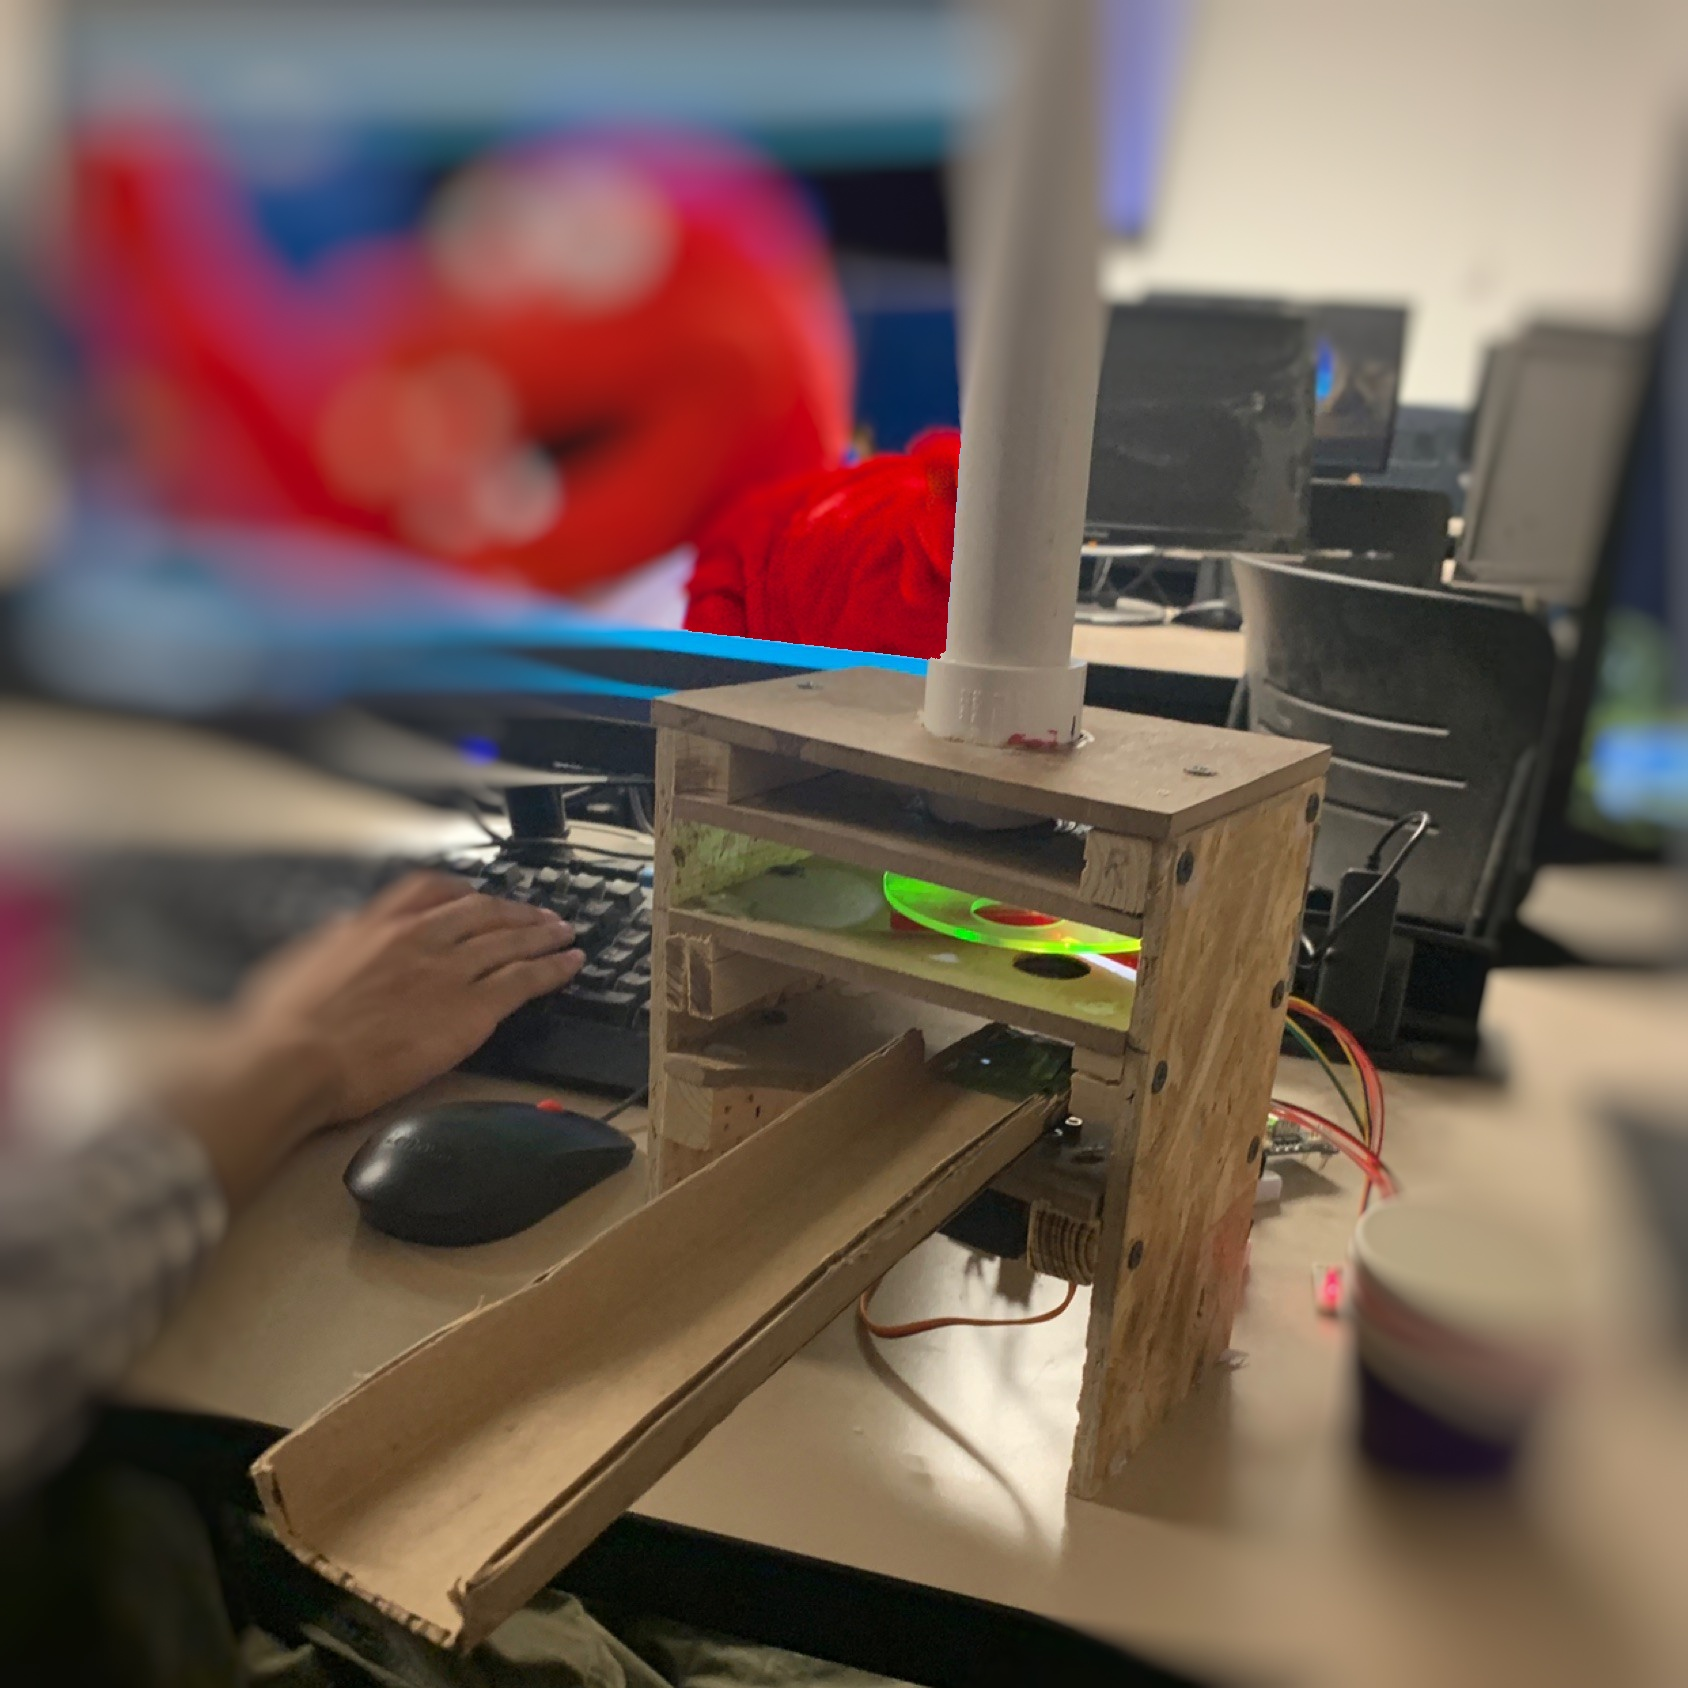
\includegraphics[width=325pt]{coverphoto-01.jpeg}\\
    \LARGE{  May 3rd, 2019. \\~\\ Team \#17 \\ The Three-Droppers \\ José Luis Gómez \\ Hammad Imam \\ Thihan Moe Kyaw \\ Daniel Spathies \\~\\ ME 250 Section \#2 \\ Professor Szwalek}
\thispagestyle{empty}
\end{center}

\newpage

\section*{Executive Summary}
The overall purpose of this project was to create a device that would sort balls by their color. This project is part of the curriculum for ME 250: Intro to Engineering Design and Graphics during the Spring 2019 semester at the University of Illinois at Chicago.\\

This report begins with an introduction on the background of the project. Next is the problem definition section, which details how the group identified constraints and objectives, and what metrics were used to define them. An objectives tree is given to detail how the group identified different objectives used in the development of the project. The problem definition section is followed by the functional analysis, which includes definitions of functions as well as a functions-means tree for the functions and means that the group brainstormed. Then, the report highlights how concepts were generated and narrowed down into the final design. The final design section is broken into mechanical, electrical, and cost subsections. The mechanical design subsection details how the physical aspects of the device were designed, from the initial sketch to a detailed CAD assembly. Dimensioned CAD drawings are provided to show more detail on the final product. The electrical design subsection describes how the components were wired and configured, and provides a wiring diagram so it can be seen how the wiring was done. It also contains a section on code which describes the main functions and algorithms used in the device. The final subsection of the final design is the cost, which provides both the dollar value of the constructed materials, and the environmental impact of the creation of the device. After the device design has been thoroughly explained, the changes and improvements made while testing are given so the stages of the design process can become clear to the reader. The report summarizes with a conclusion of the work done in the project and the lessons the group learned from working on it.\\

From the report, we can gather how a device like this might be created, going from how it was determined what it should do to how it was initially created to how it was modified to improve its performance. The major conclusions that can be drawn are that a project like this is very time consuming and requires good foresight so that nothing is unplanned for. Projects like this also require proper time management so that any issues that arise can be discovered and dealt with and still be completed in a timely manner. The major lessons learned from this project are both technical skills, as this project required coding, building, and testing knowledge that not all group members previously had; and time management skills, as many aspects of this projects went over the time constraints we had initially planned for. In the future, the group members will use these skills to improve their performance in engineering projects, both those related to academia and in industry. \\ 

Overall this project was a good learning opportunity for the team and a lot was accomplished. The device unfortunately did not have all aspects properly functional by the end of the project, but the group learned a lot through the design process and noticing what went wrong. This report aims to detail how the group went through the design process, what was changed during the design phase, and the lessons that were learned throughout the project.


\newpage
\tableofcontents

\newpage
\section{Introduction}
This tech memo is on the creation of a color sorting device that should be able to sort rubber balls by their color. This project was assigned to the team through a mechanical engineering course, the limitations in concepts, materials, and functions of the device are created by the course project guideline. Material limitations are limited to what has been listed as acceptable in one of the handouts given by the course managers and instructors. The time for the brainstorming and development of the device was also limited as it was limited to when we were told about the nature of the project. This project is the summation and an application of much of the knowledge and skills that were taught in the course. There were two projects that involved writing a technical memo on a reversed engineered device and on an experiment. They served as practice for learning how to write a technical memo. The course had CAD Solidworks, Arduino UNO, and workshop lessons which would all be applied in this project. The manufacturing of the components of the device was limited to 3D printing, the courses’ workshop materials and tools, and laser cutting. \\

The main objective of this report is to give an extensive and comprehensive explanation of the process that was taken to create the final device given the limitations and primary objective. The sub-objectives of this report, which function to accomplish the main objective, can be divided based on each section of the report. The first following section is Problem Definition, the purpose of this section is to define what the problem is in a better sense by explicitly stating the limitations of the project, creating objectives of multiple levels, and metricizing those objectives to quantify the satisfaction of those objectives. The primary culmination of this section is the objectives tree which shows all of the objectives in their order of relation and importance. The following section is Functional Analysis which is where the team begins to define what the device will perform and the possible means by which the device can perform those functions, this culminates in a Functions-means tree which gives you a layout of how the functions and means are interconnected. The next section is Concept Generation and Selection, this section is where the expansion and then contraction of ideas is done to find the best possible design concept. The expansion is done by creating a morphological chart that lists all the possible means for each of functions of the device. The morph chart is then reduced by accounting for illogical and unreliable means combinations. From the remaining possibilities a list is created of the top twenty, then one of the top five with designs images for each of them. Finally, a comparison chart of the top five concepts is created to find the top device concept. The following section is Final Design. In this section the physical design process of the top concept is explained through CAD models and explanation on modifications. The software and hardware configurations are explained in detail and finally a Bill of Materials table is created which has physical, economical, and environmental properties of each of the parts of the device, excluding hardware and software. The next section is Device Testing, this section is where the findings of trials and the decisions of modifications to the device in light of these findings are documented. The section that follows is the Conclusion of the report which should review the findings of the report, state any of the limitations of this project and suggest any improvements that could be done to this project. Finally, the report ends with References and an Appendix containing detailed information on the software used. 


\newpage
\section{Problem Definition}
\subsection{Introduction}
This section of the report is meant to define and clarify the main problem of the designing of the device. The objectives, metrics, and constraints of the designing project are stated here as they give the main context needed to define the problem. The objective tree shows all the objectives of the device in hierarchical order and grouped according to their sub-sectionality of each other. All the ideas that have been generated by the designing team have been added to the objectives tree as the purpose of the objective tree is to give a graph of all the possible objective paths that can be taken to fulfill the primary objective.1 Affinity mapping was the method used to create the objective tree. This process begins by having the objectives generated through brainstorming possible objectives and writing each one down on a sticky note. These objectives are then sorted into categories and placed according to priority.\\
The team was tasked with creating a device to autonomously sort bouncy balls by color into a predetermined number of cups. Certain considerations must be taken into account in designing such a device like using the most eco-friendly materials, manufacturing at the cheapest price and making a safe usable device that functions without input from team members.

\subsection{Definitions}
Metric: A standard of measurement; in the context of engineering design, a scale on which the achievement of a designer's objectives can be measured and assessed.
Constraint: A limit or restriction on the design’s behaviors or attributes
Objective: A feature or behavior that the design should have or exhibit

\subsection{Metrics}
Metrics are the quantification of the stated objectives, this facilitates a comprehension of the level of success of the objectives. 
\begin{itemize}
    \item Cost efficiency: cost in dollars
    \item Time Efficiency: Time in seconds
    \item User Experience: On a scale from one to ten, ten being the greatest ease of use, reusability, and transportation of the device
    \item Functionality: Based on the percentage of balls that were successfully sorted to the amount of balls to be sorted, how accurate or effective is this device at achieving its function
    \item Designer experience: Scale from one to ten, ten being the best and easiest device to construct and build.
\end{itemize}

\subsection{Constraints}
The constraints are the limitations to the means by which the device will function.The constraints for the building of this device are:
\begin{itemize}
    \item The device must be attached to the storage bin(hopper).
    \item The materials that can be used are limited to the ones found in a list.
    \item The quantity of each of the materials is limited to what is set on the aforementioned list.
    \item Energy used to power the device is limited to mechanical, electrical, and/or chemical energy.
    \item The device must be able to perform its primary objective autonomously
\end{itemize}

\subsection{Objectives Tree}
    The following diagram is the visual description of the hierarchical order, based on contribution to solving the problem,  and sub-sectionality relations of all objectives of primary, secondary, tertiary, etc., order. between all the objectives. 
    
    \begin{center}
    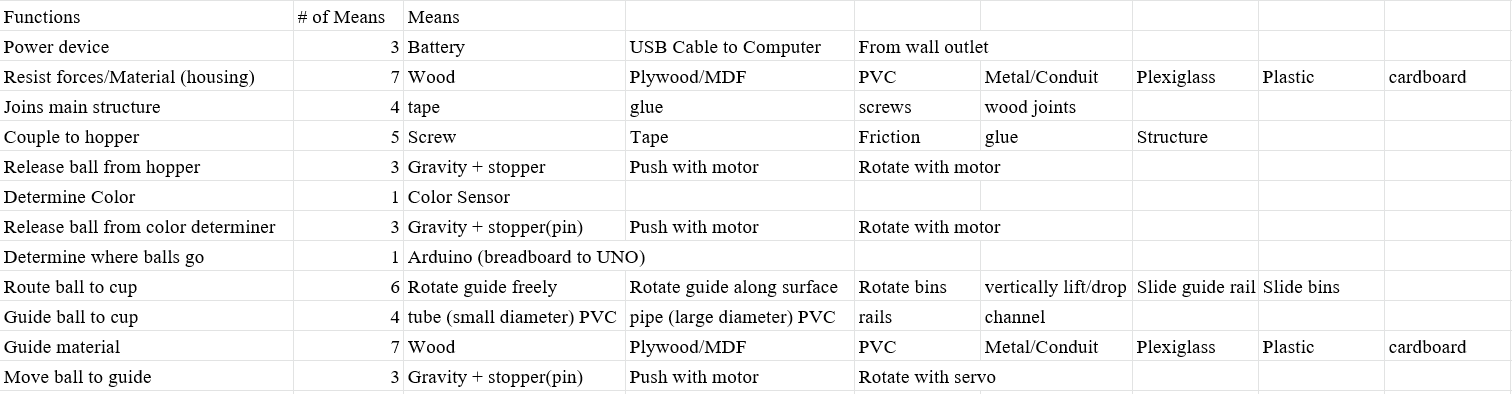
\includegraphics[width=\textwidth]{morphchart.png}\\
    \small{\textbf{Table 4.3.1} - Morphological Chart}
    \end{center}
    
    The primary objective of the device is on the top of the diagram. It is to make a machine that can sort by color. The lowered ordered objectives are objectives that can facilitate this primary objective and/or are objectives desired by the designers. These objectives have been limited to those which can be metricized for evaluation of the success of each objective for further development. The four main secondary objectives are efficiency, user experience, designer experience, and functionality. Under these objectives there are multiple objectives that are subsections of these four secondary objectives.
    It should be noticed that none of the objectives in the objectives tree are necessary elements of the device. This is due to the clear distinction between objectives and constraints, as they are defined above. There is only one primary objective which is the main answer to the problem statement.

\subsection{Conclusion}
To conclude this section, the metrics, constraints and objective tree are the parts of this section which give the context of the problem, something important for final analysis on determining how to go about solving the problem. The objective tree is important for understanding the hierarchical order and subsectional relationships of the objectives. The metrics and constraints sections of this section are also important as they help the designer understand what they are limited to and how it is that they can evaluate the success of their objectives. 

\newpage
\section{Functional Analysis}
\subsection{Introduction}
This section is on the functions and means of the device. The primary functions that the device is supposed to perform as well as the sub functions that the corresponding means will need are listed. The meaning of functions and means as they are used in this report refer specifically to engineering design and so are defined in this section for clarification. The functions and means are presented in a tree diagram which is meant to highlight the ranking of importance/order of the functions and link the means to their corresponding function.
\subsection{Definitions}
(Basic/Primary) Functions- what a device is supposed to do, should be described using verbs.
Means- The ways by which primary functions can be implemented, should be described using
nouns.
Secondary/sub functions- Functions that are governed by the means of the basic functions[2].
\subsection{Function-Means Tree}
The function-means tree is meant to give order to all the types of functions and their corresponding means. The order is based on the purpose of the function. Functions that serve the purpose of mitigating or completing other functions are secondary functions. All others are basic primary functions. Figure 3.3.1 is the functions mean tree for this projects device. The tree starts by giving primary functions in bolded text in rectangular boxes. More specific functions that explain the pieces of the primary functions are then given in underlined text in rectangular boxes. Means for each function are in plain text trapezoidal boxes below each function. Additional sub functions specific to each means are then given in plain text in rectangular boxes. \\

Tree outline

\begin{itemize}
    \item \textbf{Power Device}
    \item \textbf{Contain Structure}
        \begin{itemize}
            \item Resist forces
            \item Join main structure
        \end{itemize}
    \item \textbf{Load balls in from hopper}
            \begin{itemize}
            \item Couple from hopper
            \item Release balls from hopper
        \end{itemize}
    \item \textbf{Sort by color}
            \begin{itemize}
            \item Determine color
            \item Release from color determiner
        \end{itemize}
    \item \textbf{Send ball to cup}
            \begin{itemize}
            \item Determine where balls go
            \item Aim ball to cup
            \item Move ball to guide
            \item Guide ball to cup
            \item Resist forces while guiding ball
        \end{itemize}
\end{itemize}

\begin{center}
    
\includegraphics[width=420px]{functionmeans.png}\\
    \small{\textbf{Figure 3.3.1} - Functions-Means Tree}\\
    \small{Full size available \href{https://raw.githubusercontent.com/himam99/ME250-Proj3/master/LaTeX/Images/functionmeans.png}{here.} }
\end{center}

\newpage
\section{Concept Generation}
\subsection{Introduction}
This section’s purpose is to present the procedure that was taken to select the concept design for the color sorting device. In this section, a morphological chart is used to generate all the possible design concepts by listing all the functions and their corresponding means. From this the top twenty or so concepts are chosen through an analysis on their practicality and ability to satisfy objectives. These concepts are listed in this section. From this a list of the top five concepts are chosen through more rigorous application of the same analysis as beforehand, these top five are also listed and justified. Finally, through the use of comparison charts the top concept is selected for manufacturing the device.

\subsection{Definitions}
Morphological chart: A matrix in which the leftmost column is a list of all of the principal functions that our design must perform and also some of the key features it must have. \\
Design space: An imaginary intellectual region of design alternatives that contains all of the possible solutions to the design problems[3].

\subsection{Morphological Chart}
The leftmost column of the chart shows the functions that should be included in the design. To the right of the functions are the all different types of means that were found which could perform the functions. The purpose of this chart, Figure 4.3.1 is to aid in expanding the design space.

\begin{center}
    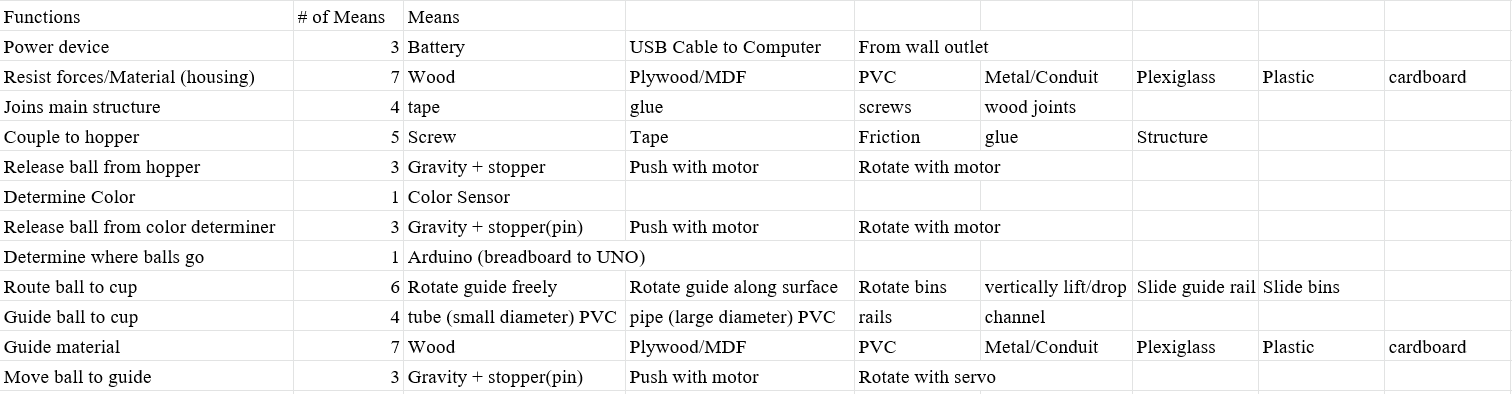
\includegraphics[width=\textwidth]{morphchart.png}\\
    \small{\textbf{Table 4.3.1} - Morphological Chart}\\~\\
    
    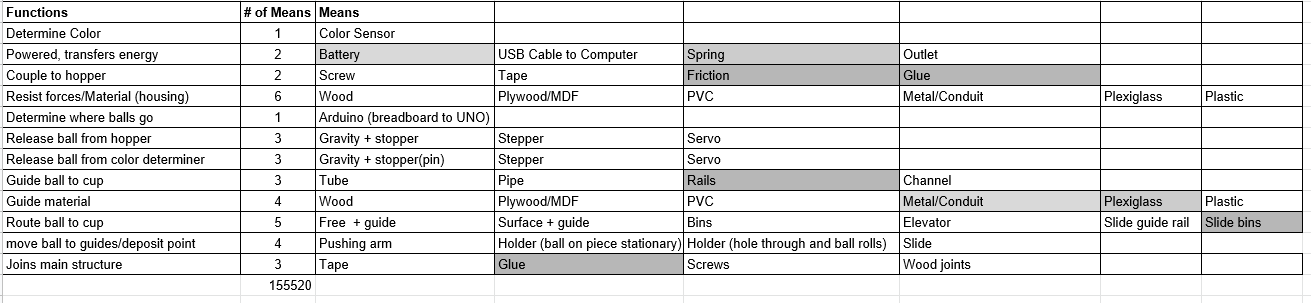
\includegraphics[width=\textwidth]{morphchartreduced.png}\\
    \small{\textbf{Table 4.3.2} - Reduced Morphological Chart}\\~\\
    
\end{center}

For Figure 4.3.2, the majority of the reductions in means are ones that are unreliable and impractical both relative to other means and somewhat objectively. For example, glue is not strong enough to withstand the forces on the main structure, so it was eliminated from the morph chart.

\subsection{Concept List}

\begin{itemize}
    \item   Wood housing using screws as main joiner, the color sorter is under the hopper, the ball then drops on an arm attached to a servo. The servo then rotates the calculated amount to one of the three fixed pvc pipes that lead to a cup.
    \item Cardboard housing using duct tape as main joiner, after color is sensed, a cardboard     channel is moved by a servo to align with the proper cup and then the ball is released from the color determining area and then goes down the channel into the correct cup
    \item Wood housing with screws as main joiner, also there are fixed ramps made of cardboard, the ball moves from hopper to color sensor, then the ball gets released and gets deviated dependant on arduino code to go down a different ramp which will lead to a corresponding cup 
    \item PVC housing with glue and tape as main joiners, this device acts as an elevator or dumbwaiter, after determining the color at the top of the shaft, this device drops the ball a determined height into the right cup, a servo with string can be used to lower or raise elevator shaft to desired position.
    \item Wooden housing with plastic, a spring and glue or tape as joiners, this device brings a ball from the hopper to the color sensor then drops it into a waiting catapult arm with a spring attached. The arm is pulled back at the precise distance to allow the ball to fly as a projectile and land in the correct cup, the arm is then winched back with a motor to an arduino determined distance and repeated.
    \item Wooden housing, a type of manufactured belt, metal to make conveyor and cardboard with various joiners being required. First, a single ball is deposited from the hopper and dropped onto a rotating conveyor belt that moves the ball to the right, the ball passes under the color sensor and the color is determined and then the arduino and code process the color and move a moveable ramp/platform at the end of the conveyor to bounce the ball into the correct cup.
    \item Wooden housing, a type of manufactured belt, metal to make conveyor and cardboard with various joiners being required. Similar to the other device using a conveyor, this device releases a ball onto the moving conveyor belt, scans the color and continues down the conveyor but next one of three motors is turned on and when it senses motion, extends to push to ball off the side of the conveyor into the correct cup.
    \item Wooden housing with screws or tape as main joiner, after scanning the color of the ball in the color scanning portion of the device, the ball is then dropped onto a ramp with a very small slope or angle and as the ball slowly travels down the ramp, the servo corresponding to the correct cup then moves and opens a hole for the ball to fall through into the cup below it
    \item Wooden housing with screws as main joiner, after ball’s color is sensed, the ball drops onto an arm attached to a servo, the arm rotates to be over the correct cup and then the servo on the arm activates, opening a hole in the arm, releasing the ball into the correct cup
    \item   Cardboard housing with glue and tape and main joiners, the ball gets released from hopper, color gets sensed and then after being released from the color sensing station, the ball is redirected by a servo with an extended arm to push the ball down of of the three separate paths of the connected ramp into the desired cup
\end{itemize}

\begin{center}
    Top 5 Concepts
\end{center}



\begin{itemize}
    \item Tri-Tube -  Wood housing using screws as main joiner, the color sorter is under the hopper, the ball then drops on an arm attached to a servo. The servo then rotates the calculated amount to one of the three fixed pvc pipes that lead to a cup.
    \item Moving channel -   Cardboard housing using duct tape as main joiner, after color is sensed, a cardboard channel is moved by a servo to align with the proper cup and then the ball is released from the color determining area and then goes down the channel into the correct cup
    \item Conveyor belt -  Wooden housing, a type of manufactured belt, metal to make conveyor and cardboard with various joiners being required. First, a single ball is deposited from the hopper and dropped onto a rotating conveyor belt that moves the ball to the right, the ball passes under the color sensor and the color is determined and then the arduino and code process the color and one of three motors pushes the ball when motion is sensed into the correct cup
    \item  Arm controller - Wooden housing with screws as main joiner, after ball’s color is sensed, the ball drops onto an arm attached to a servo, the arm rotates to be over the correct cup and then the servo on the arm activates, opening a hole in the arm, releasing the ball into the correct cup
    \item Tri-fold ramp- Cardboard housing with glue and tape and main joiners, the ball gets released from hopper, color gets sensed and then after being released from the color sensing station, the ball is redirected by a servo with an extended arm to push the ball down of of the three separate paths of the connected ramp into the desired cup
\end{itemize}

\subsection{Top 5 Drawings}

\begin{center}
    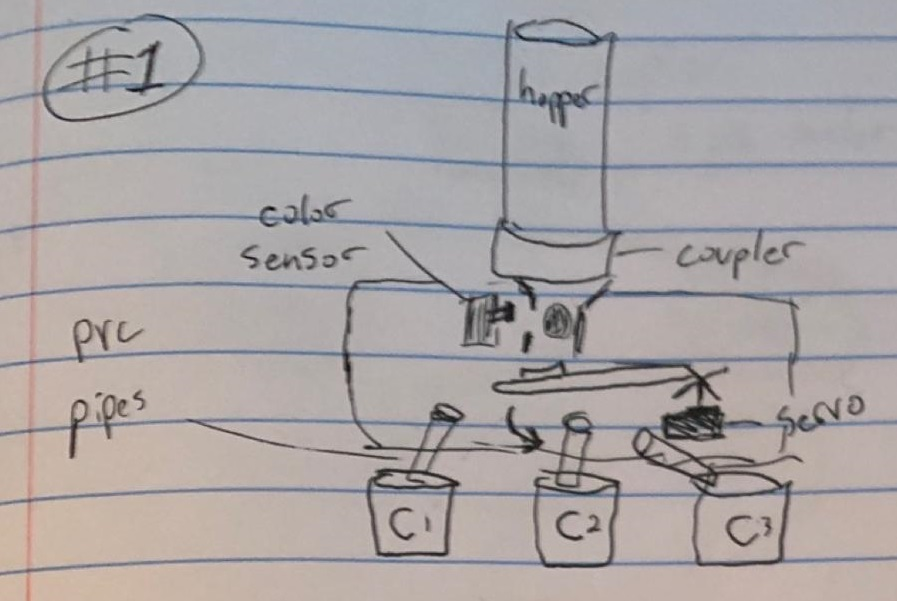
\includegraphics[width=400px]{cg_1.jpg}\\
    \small{\textbf{Figure 4.5.1} - Tri-Tube}\\~\\
    
    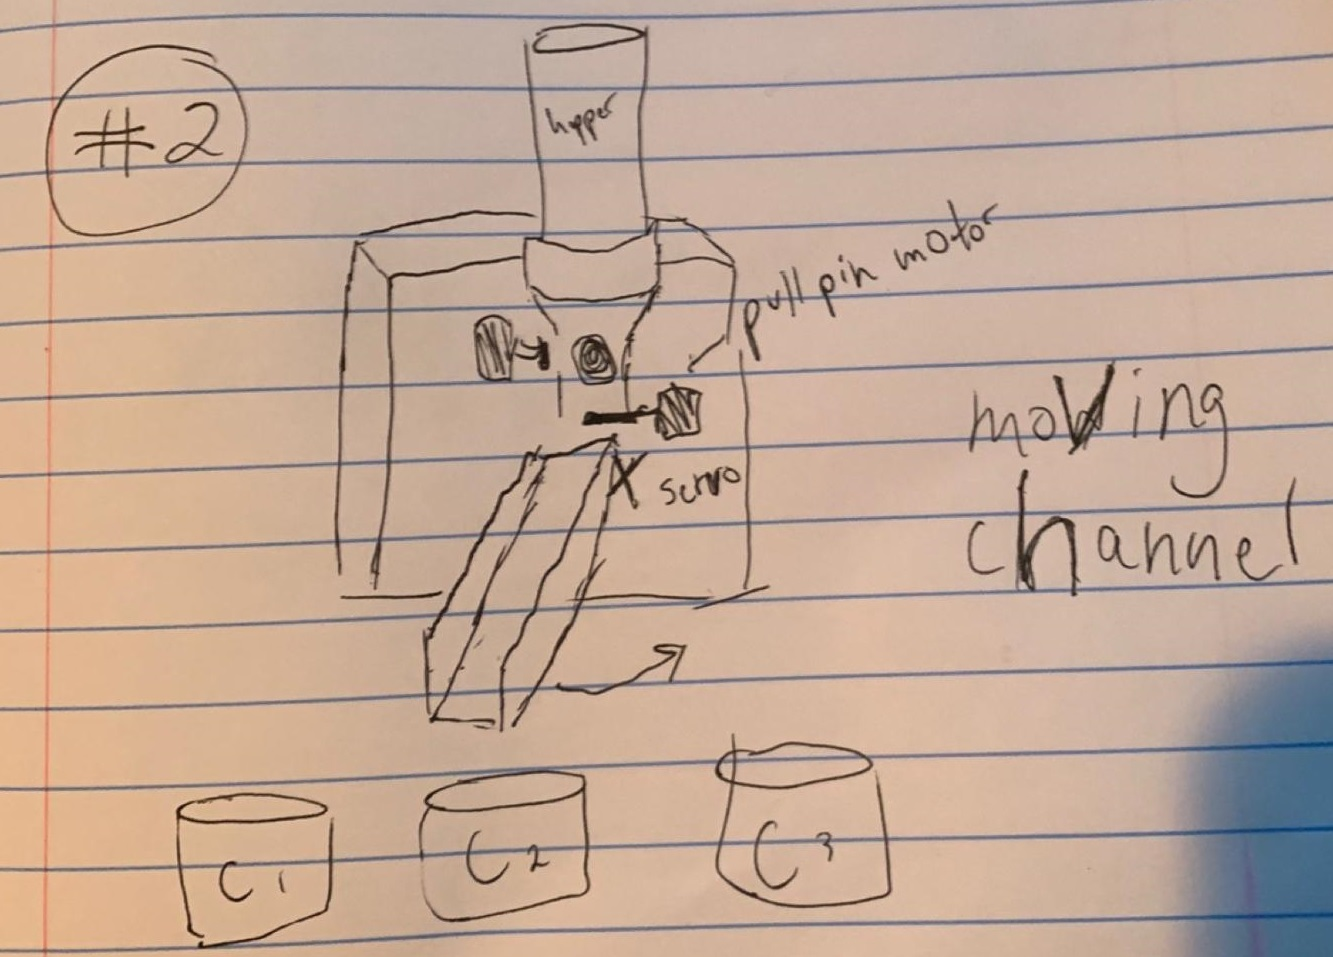
\includegraphics[width=400px]{cg_2.jpg}\\
    \small{\textbf{Figure 4.5.2} - Moving Channel}\\~\\
    
    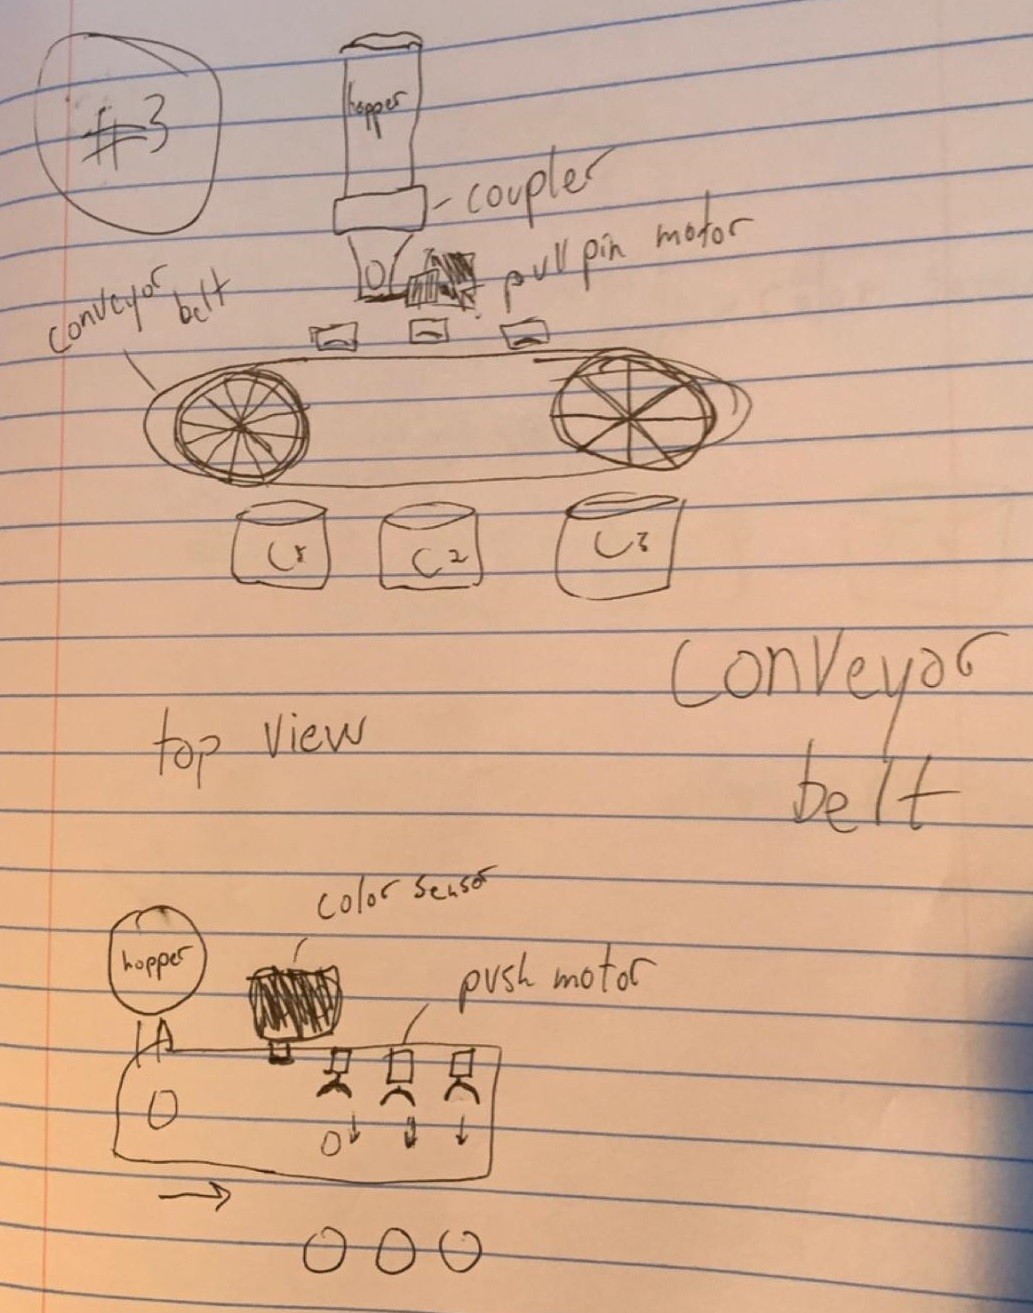
\includegraphics[width=\textwidth]{cg_3.jpg}\\
    \small{\textbf{Figure 4.5.3} - Conveyor Belt}\\~\\
    
    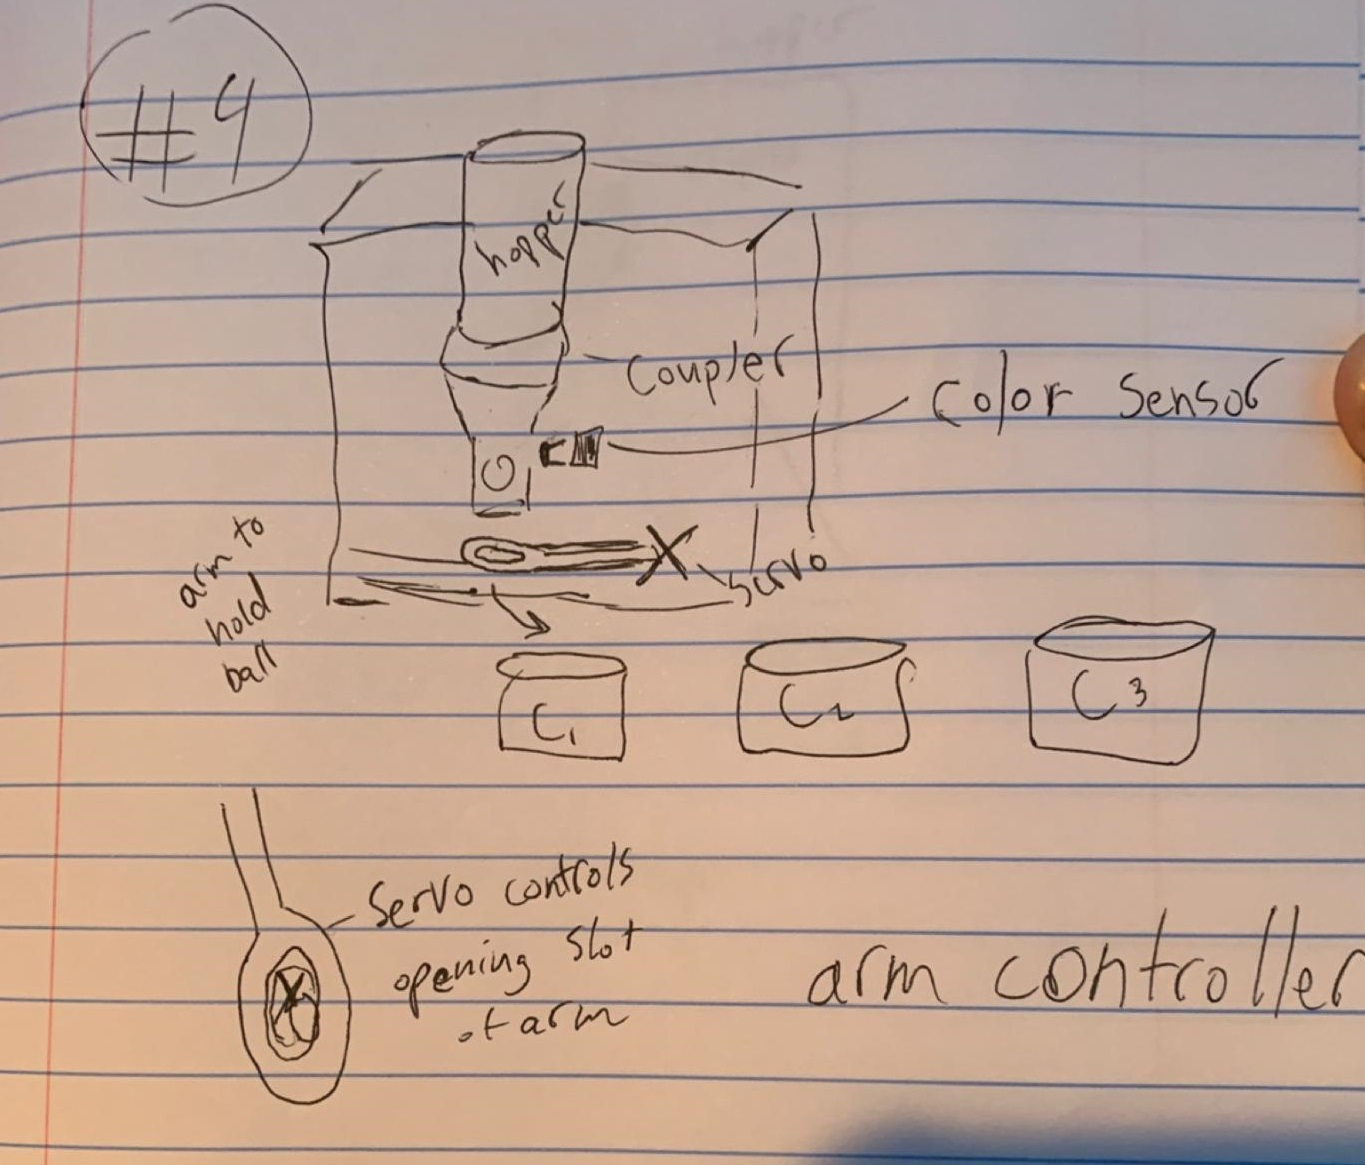
\includegraphics[width=\textwidth]{cg_4.jpg}\\
    \small{\textbf{Figure 4.5.4} - Arm Controller}\\~\\
    
    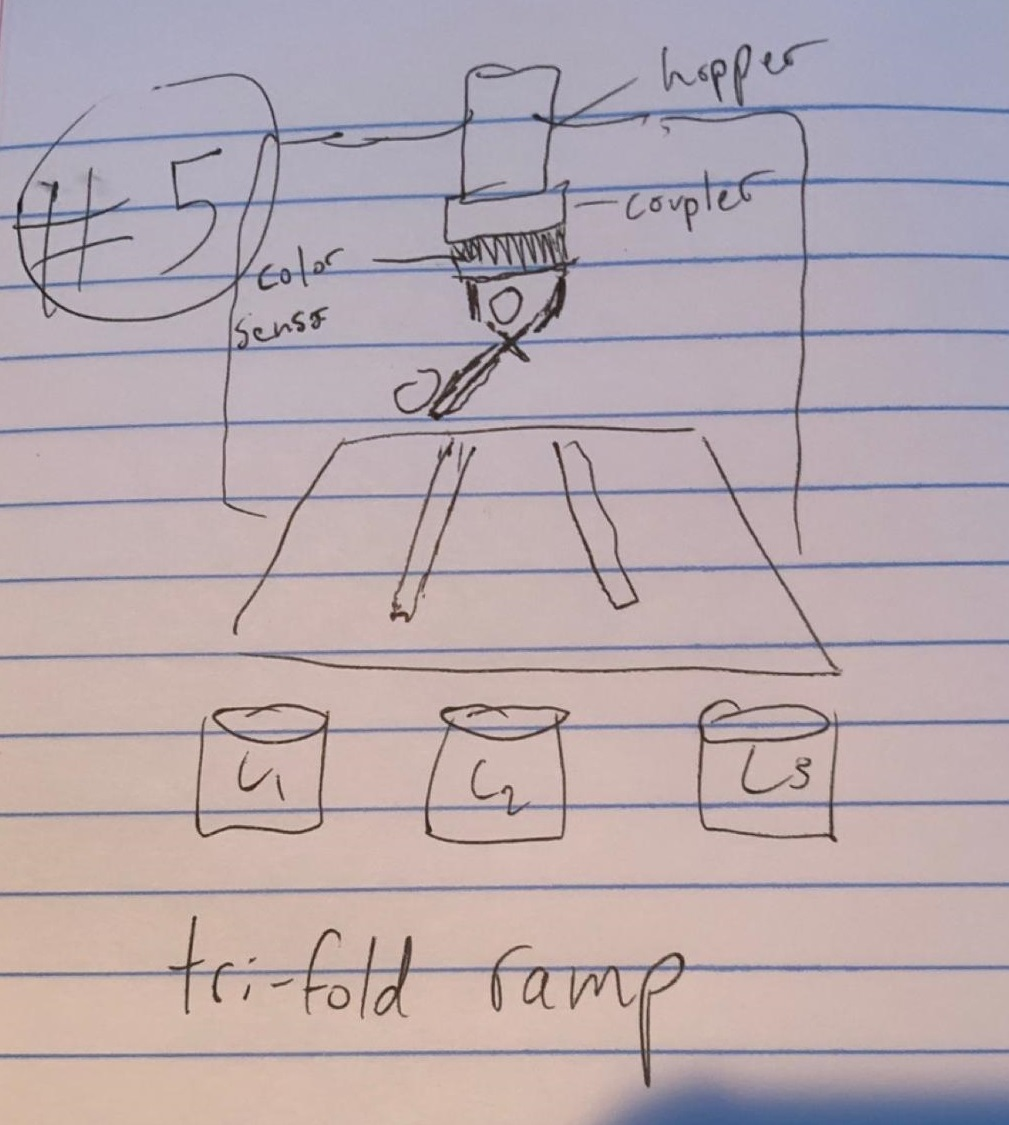
\includegraphics[width=\textwidth]{cg_5.jpg}\\
    \small{\textbf{Figure 4.5.5} - Tri-fold Ramp}\\~\\
    
\end{center}

\subsection{Comparison Chart}

\begin{center}
        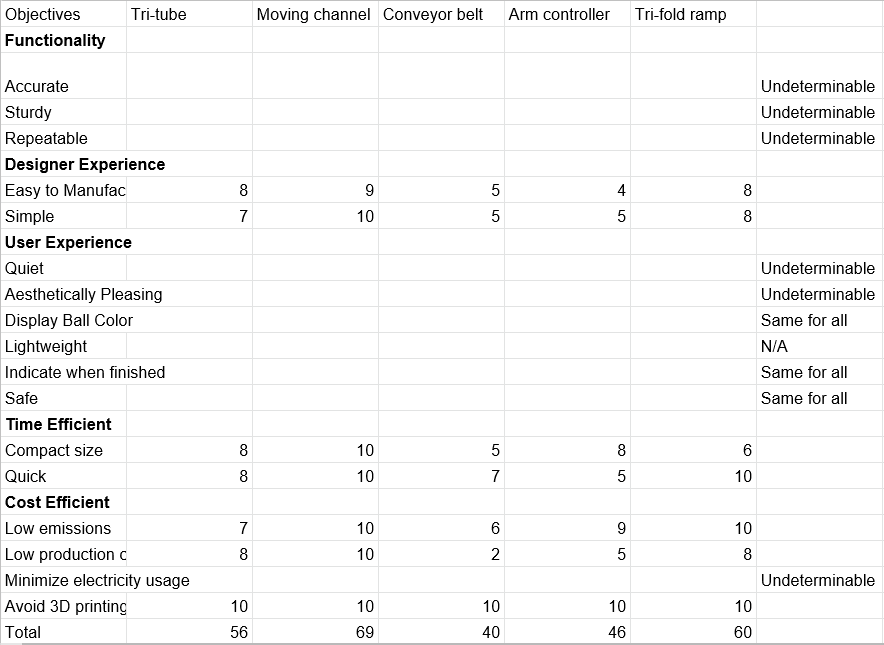
\includegraphics[width=\textwidth]{comparisonchart.png}\\
    \small{\textbf{Table 4.6.1} - Comparison Chart}\\~\\
\end{center}

The above chart, Table 4.6.1, was used to compare the top five concepts to select the top three designs and the best design. Each objective that could be determined from the initial designs was ranked from 1-10 with 10 being the highest. The scores were then summed, with the top design being the one one the highest sum. \\
Many of the objectives were given a rating of "Undeterminable" if it was not possible to determine from the initial design. Notably, there was some difficulty in finding the appropriate way to predict many of the secondary objectives in the functionality objective. Other objectives were given a rating of "Same for All" or "N/A" if it was determined that all designs would perform roughly the same for that objective.

\subsection{Conclusions}

In accordance with the purpose of this section, the most important parts of this section are the morphological chart, the comparison chart and the concepts lists and explanations for reductions in means. The morphological chart is of great importance as it is what is primarily used in order to generate all the different types of concepts. The explanations of the process taken to reduce the number of possible concepts is of great importance as it is how we come to closer to a limited amount of concepts. The comparison chart is of great importance as well as it presents the rankings that we performed in evaluating the best concept. Using the comparison chart we ultimately arrived as the moving channel concept as being the best as it ranked best in cost and time efficiency and was also the top performer in the objective of designer experience. This design was chosen to be our final design and will be detailed more thoroughly in the `Final Design' section.


\newpage
\section{Final Design}
\subsection{Introduction}
This section documents how the design was created from the original concept. The first subsection is the mechanical design, which details how we came up with the physical construction of the device, how we designed it with CAD, and how we created it; it includes CAD drawings of the design at different stages of development and explanations and rationale for why those changes were made. The second subsection is the electrical design, which contains detailed explanations of both how the hardware was configured and how the software was designed; to illustrate the electrical design, both a photograph and wiring diagram of the circuit are provided. Finally, the third subsection is the cost, which breaks down how expensive the device was to produce, based on both a bill of materials with dollar value and an environmental impact report that finds the footprint of each individual component.
\subsection{Mechanical Design}
\subsubsection{Preliminary Design}
The team wanted to minimize the materials used and use materials that were as cost effective as possible. Keeping in mind that the hopper would be able to be suspended above the device, the team decided to use a gravity fed device that would take one ball at a time, drop it into a rotating plate connected to a stepper, scan the color of the ball, drop it through a hole into the next sub level and then the ball would drop onto the ramp which is connected to a servo motor that rotates the ramp to be above the correct cup. This design incorporated MDF wood for the housing, screws and glue as the joiners and cardboard, wood and PVC for the internals. Using the Arduino and a color sensor, the device is able to sense and redirect a ball to the correct cup. The device was built hoping to achieve the objectives as efficiently as possible. 


\begin{center}
    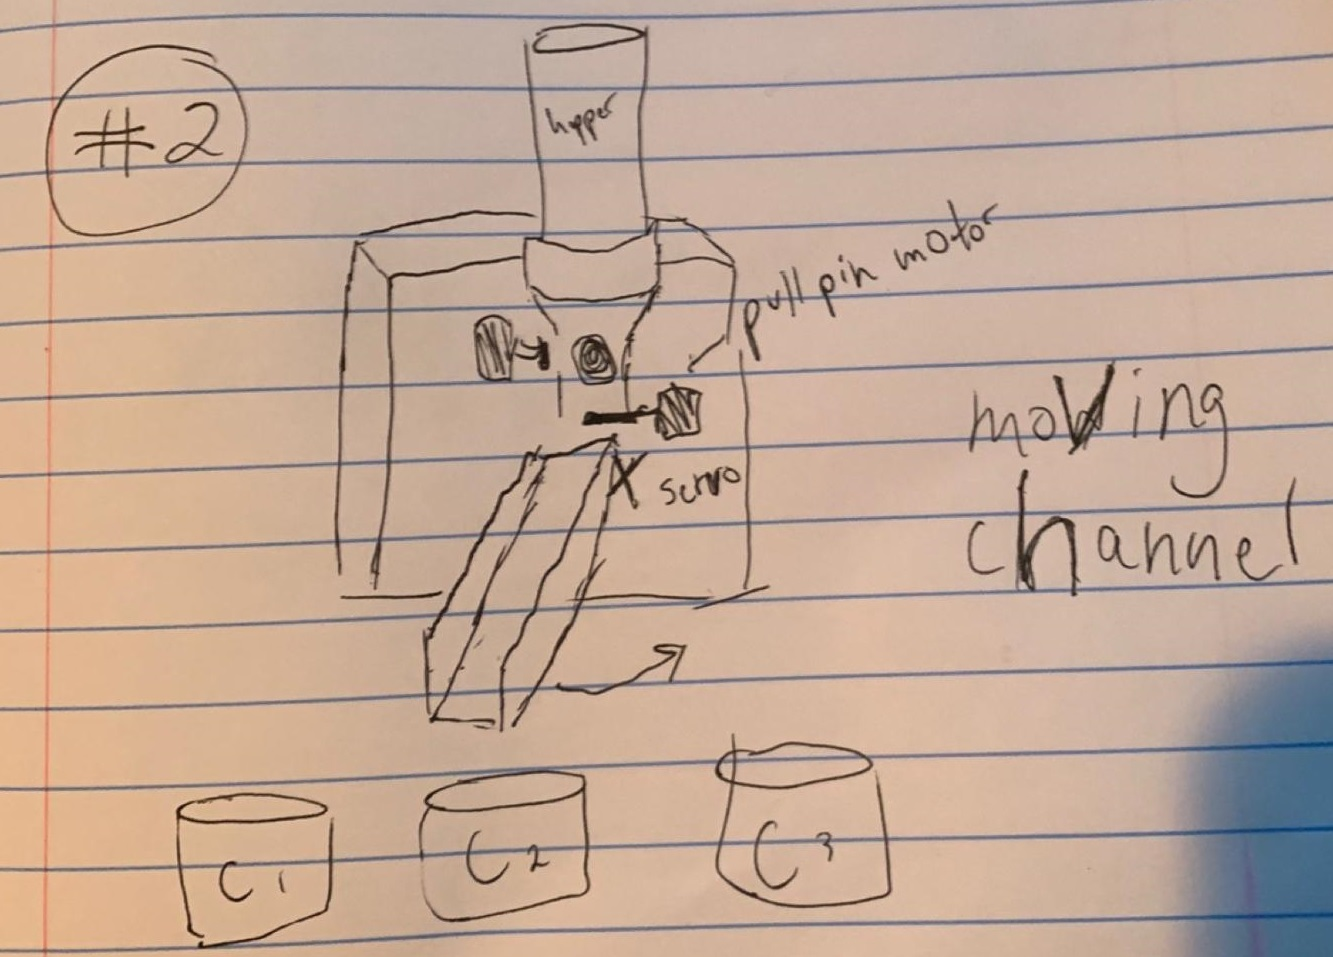
\includegraphics[width=400px]{cg_2.jpg}\\
    \small{\textbf{Figure 5.2.1.1} - Moving Channel}\\~\\
\end{center}

\subsubsection{Prototype}

This design was the first attempt at recreating the idea from the drawing in CAD. The device is made mainly using 1/8" plywood, except for the stepper horn which is 3D printed. The top plate of the device has a large hole which can hold the outside diameter of the hopper, followed by a plate with a small hole that does not let the hopper tube pass through but lets the balls through. Below that, a stepper motor rotates a plate with 3 holes. This middle plate is close enough to the hole that a ball cannot drop down from the upper plate unless the hole in the wheel is aligned with the hole in the upper plate. The wheel then rotates the ball along the middle plate until is next to the color sensor, which detects the color of the ball and sends it to the Arduino. Next, a servo motor attached to the ramp via a ramp bracket rotates so that the ramp points towards the correct bin. The wheel rotates again, which simultaneously loads in another ball, rotates the previously loaded ball to the scanner, and rotates the just-scanned ball to a hole in the middle plate where it will fall onto the ramp and roll into the correct bin. The lower plate has a hole cut to house the servo, as well as a small round cut in the side of it so that the ramp has a wider range of mobility before it hits the plate. The pieces were mostly to be glued together to avoid the need for lots of fasteners such as screws and bolts. Overall the prototype design was a first draft at realizing the initial drawing and helped us conceptualize how our design would work before we built it.

\begin{center}
    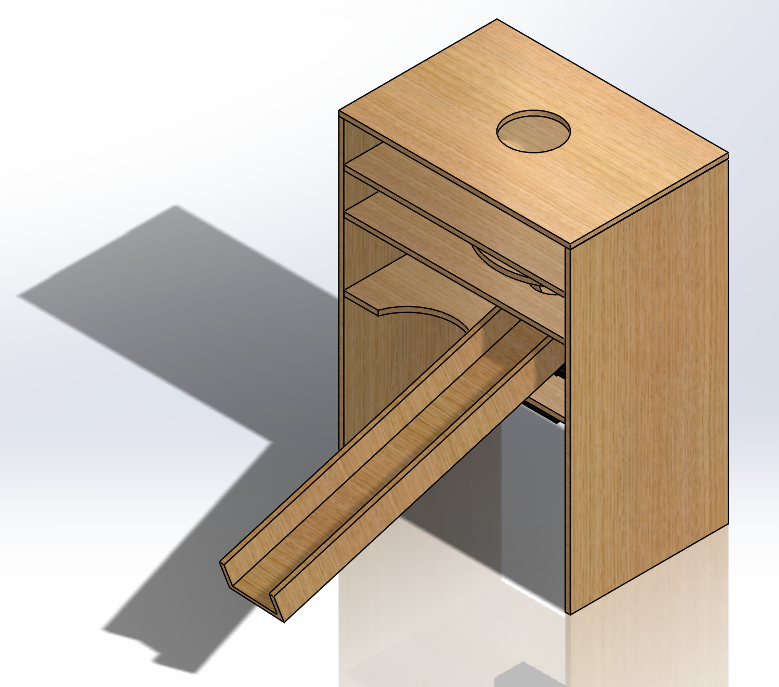
\includegraphics[width=\textwidth]{assembly_OLD.png}\\
    \small{\textbf{Figure 5.2.2.1} - Prototype CAD Assembly}\\~\\
\end{center}

\subsubsection{``In Progress" Redesign}

This design was created after the initial design when the group moved from the designing phase to the building phase. The most notable change was that all the wood pieces are now made of 1/4" wood instead of 1/8" like the original design, and the wheel is made of 1/8" laser-cut acrylic instead of hand-machined plywood. The wood was changed to 1/4" plywood both because the group determined 1/8" may not be sturdy enough, and because the lab did not have a large enough supply of 1/8". The wheel was switched to laser-cut acrylic since the group determined it would be too time consuming to accurately cut a circular wheel by hand. Overall, the design remained mostly the same, with only some changes made to better reflect the work environment that the group had access to.

\begin{center}
    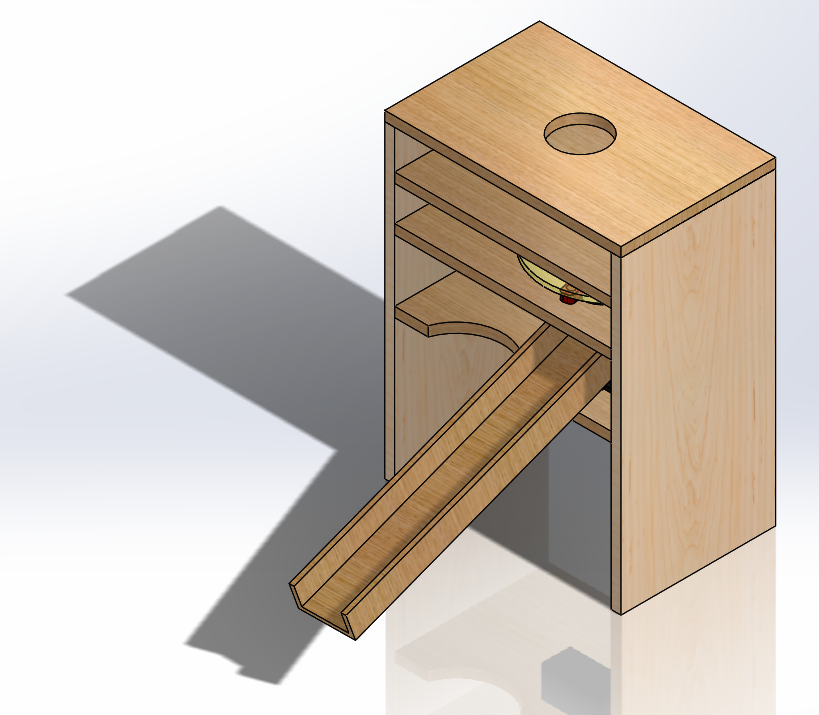
\includegraphics[width=\textwidth]{assembly_IP.png}\\
    \small{\textbf{Figure 5.2.3.1} - ``In Progress" CAD Assembly}\\~\\
\end{center}

\subsubsection{``As Built" Design}

The ``As Built'' design is notably different from the previous iterations. The most drastic change is that the pieces are now attached using screws instead of glue, which required some mild redesigning. The materials used were primarily OSB and MDF, which both would not hold well if a screw was drilled into the side. To fix this problem, supports were created out of 2x4s, which then had holes drilled into them to attach the pieces together at right angles. To space the section with the wheel properly, the upper plate was moved to be flat against the same support beams used for the top plate. Other small changes included the ramp material changing from plywood to cardboard since it was easier to create and weighed less, causing less strain on the servo. The color sensor was also relocated from the side wall to above the wheel so that it could get a more accurate reading as well as being more easily mounted and managed. The hole in the upper plate was widened to make room for a PVC coupler that could hold the hopper, as well as featuring a diversion ramp that ensured the ball was in the correct spot.

\begin{center}
    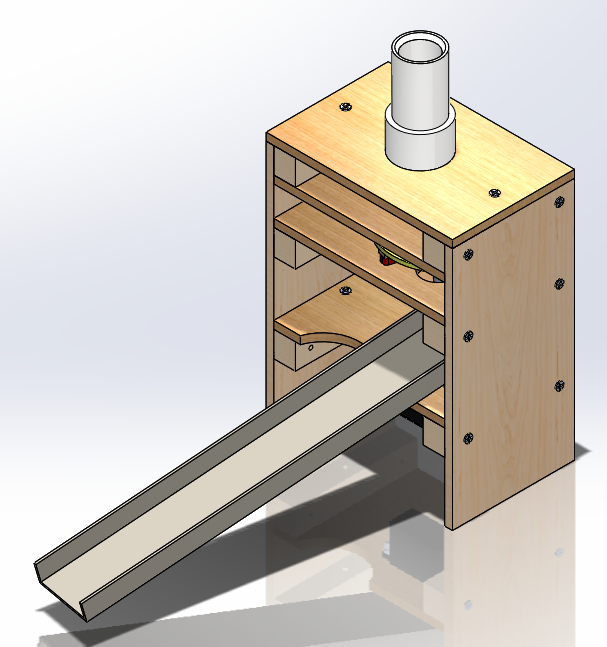
\includegraphics[width=\textwidth]{assembly_AB.png}\\
    \small{\textbf{Figure 5.2.4.1} - ``As Built" CAD Assembly}\\~\\
\end{center}


Screenshots of dimensioned CAD drawings are available below since this was the final iteration. For the CAD files of other development stages, or for the full sizes of these drawings, see Appendix C.

\begin{center}
    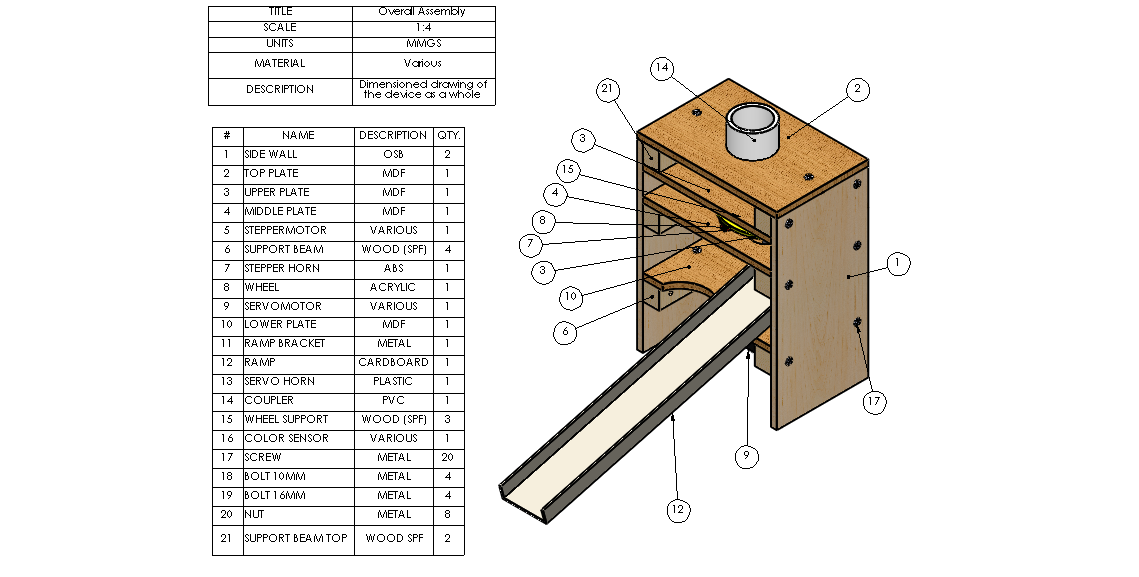
\includegraphics[width=\textwidth]{assemblyandBOM.PNG}
    \small{\textbf{Figure 5.2.4.2} - Assembly with Bill of Materials}\\~\\
    
    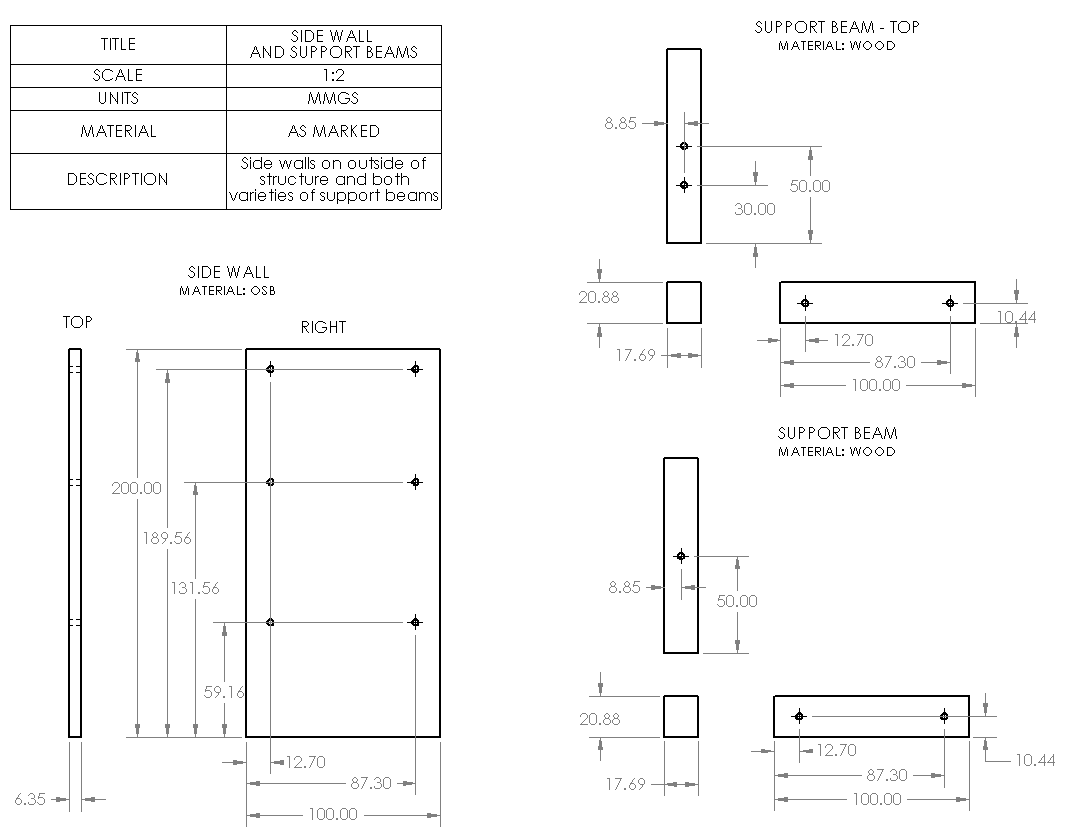
\includegraphics[width=\textwidth]{sidesupport.PNG}
    \small{\textbf{Figure 5.2.4.3} - Assembly with Bill of Materials}\\~\\
    
    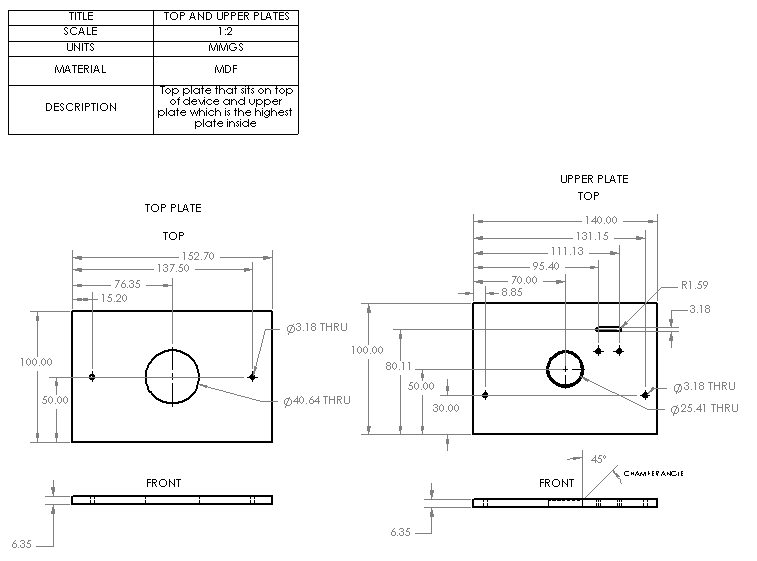
\includegraphics[width=\textwidth]{topupper.PNG}
    \small{\textbf{Figure 5.2.4.4} - Top and Upper Plates}\\~\\
    
    \includegraphics[width=\textwidth]{midlowerplate.PNG}
    \small{\textbf{Figure 5.2.4.5} - Middle and Lower Plates}\\~\\
    
    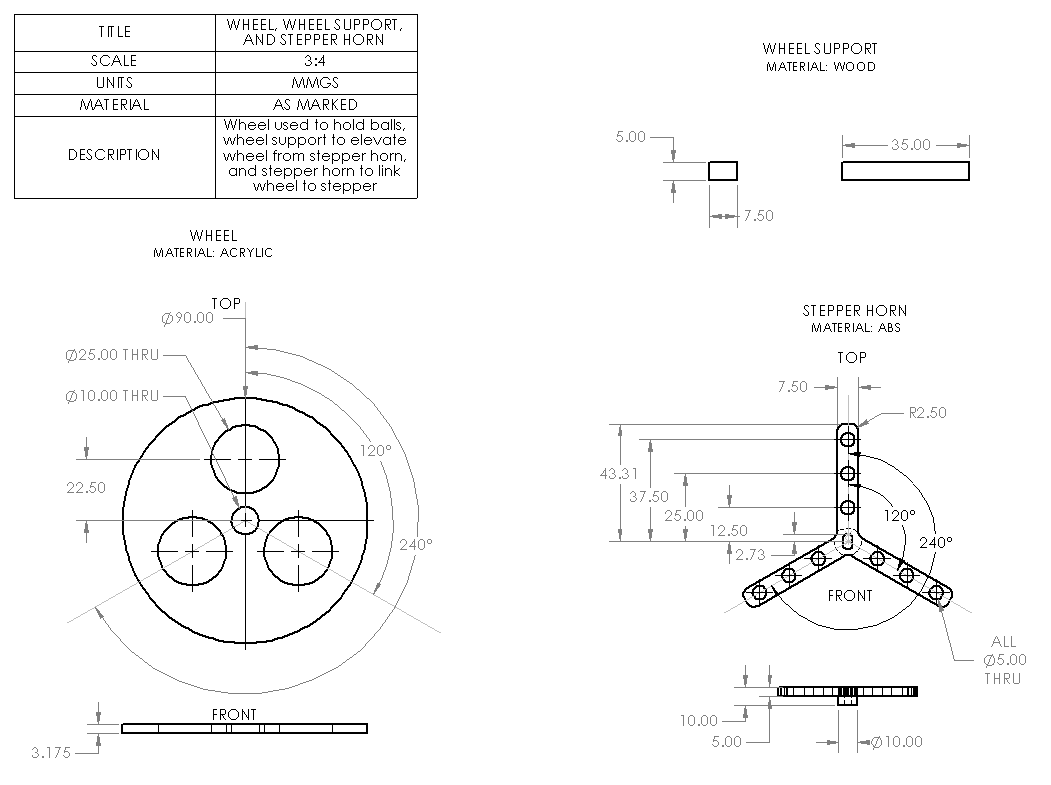
\includegraphics[width=\textwidth]{wheelstepper.PNG}
    \small{\textbf{Figure 5.2.4.6} - Assembly with Bill of Materials}\\~\\
    
    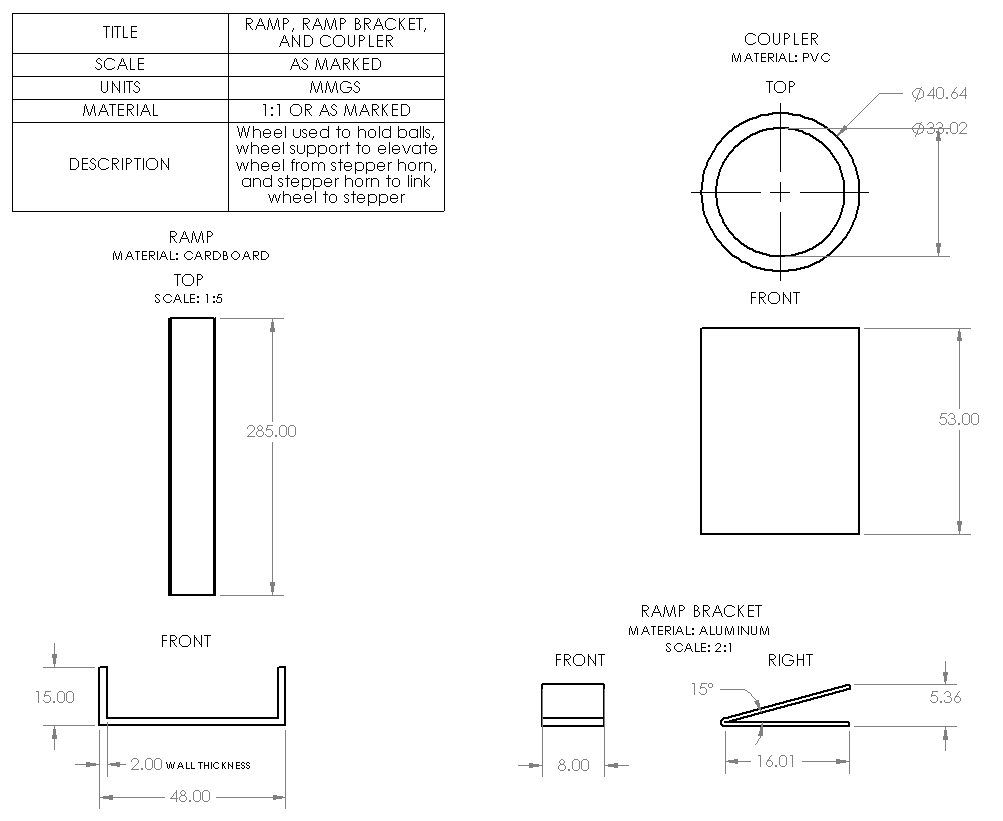
\includegraphics[width=\textwidth]{rampcoupler.PNG}
    \small{\textbf{Figure 5.2.4.7} - Assembly with Bill of Materials}\\~\\

\end{center}

    
\newpage
\subsection{Electrical Design}
\subsubsection{Hardware}

    The following section will describe the hardware used for the project. The table 5.3.1.1 shows the quantity of hardware and the description of each piece, and figure 5.3.1.2 shows a circuit diagram of the hardware.
    
    \begin{center}
    \begin{tabular}{|c|c|c|c|}
    \hline
       \textbf{\#}  & \textbf{Name} & \textbf{Qty} & \textbf{Description}  \\
       \hline
        1 & Arduino & 1 & Controls the device\\
        2 & Small breadboard & 2 & Connect hardware\\
        3 &  RGB LED & 1 & Shows signals from Arduino\\
        4 & Stepper Motor & 1 & Rotates wheel \\
        5 & Servo Motor & 1 & Rotates ramp \\
        6 & Resistor & 1 & 10k$\Omega$, protects LED from blowing out\\ 
        7 & Color Sensor & 1& Reads color value \\
        8 & Power Supply & 1 & Supplies power to motors\\
        \hline
    \end{tabular}\\
    \small{\textbf{Table 5.3.1.1} - Circuit Materials}\\~\\
    
    \end{center}
    
    \begin{center}
    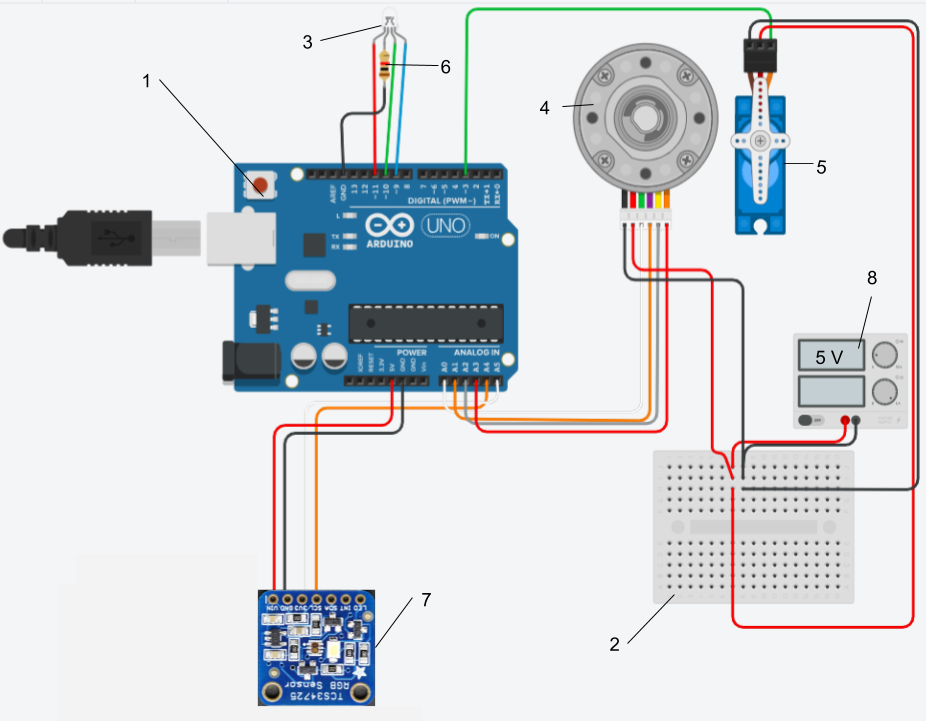
\includegraphics[width=300px]{circuit.png}\\
    \small{\textbf{Figure 5.2.4.2} - Circuit Diagram}\\~\\
    \end{center}

The hardware was designed to be as minimalist as possible given what was necessary. Our design called for one form of stepped continuous rotation and one form of motion that set an angle, so one stepper and one servo were used. The TCS sensor was used to sense the color of the ball. An RGBLED was also used for signalling so that the process could be displayed to the user. The TCS and RGBLED ran off the power provided by the Arduino, while a separate 5V DC power supply was required to run the motors. The circuit design originally did not include the power supply, but there were issues with power draw that neccessitated the addition of the power supply. Other than that, no other modifications were made to the circuit design since the start.

\newpage
\subsubsection{Software}
The software for this project was written in two attempts. The first attempt was a prototype code and largely consisted of a long string of if-elseif-else statements that would check if the ball was within a certain color value and then set the servo to route the ball to the correct spot. While it's possible this code could have functioned properly, it was hard to configure since the values that would need to be changed were in different places, and it used a confusing system of boolean variables. Additionally, this code could only be configured for option A and the group had decided to try option B. Ultimately this code was not used in the final testing.\\

The second version of the code was much more streamlined, and used custom functions. It began with a "config" section that had all the pins that needed to be used and all variables that were used in the body of the code. Then, the setup() section was used to set up pins and initialize motors and the color sensor. The void() section was the main part of the code, with a for loop used to check the sensed color against stored variables to determine what color the ball was, and a nested for loop to check the bins for which places needed what balls and to route the balls there. Multiple functions were custom defined for the sake of saving space while writing the code. This also proved to be very useful since longer processes that needed to be repeatedly written, such as making the LED blink, were simplified into a single function that could be called with much less typing. More detail on the code is given below.\\

A unique aspect of the software used for this project was that a custom struct called "ballColor" was defined. Each color ball had its own ballColor that contained the color name as a string, an array with expected RGB values from the color sensor, and an array with RGB values to display on the RGBLED. The structs were then compiled into an array called "balls" so that balls[0] could call the first ball struct, balls[1] could call the second ball struct, and so on. This process was repeated for the bins with a struct called bin\_type so that the bins could be called in a similar fashion. The code uses this process so that the code could use a for loop to iterate through all balls instead of each ball needing to be typed out in the code.\\

To start, a function called checkColor() was written to simplify checking the color of the ball. The function would compare the color of the sensed component to a stored array for red, blue, and green values. If all 3 conditions were met, then the function would return true. This function was used as a quick way to check ball colors since checking these values one at a time would take a longer time. By writing this function, checking a ball color was able to be the condition for an if statement which made it much easier to check the ball color.

\begin{center}
    \includegraphics[width=\textwidth]{code_1.png}\\
    \small{\textbf{Figure 5.3.2.1} - checkColor() function}\\~\\
\end{center}

The code also used two functions for RGB output. The first was colorWrite(), which took an array of RGB values and displayed them on the RGBLED using 3 analogWrite() functions. The second function was colorBlink(), which took an array of RGB values and an integer. colorBlink() would pass the array to the colorWrite() function and turn the LED on and off for 250ms each for the number of times that it was given. These functions were used to signal with the RGBLED what was going on with the device. Integer arrays for red and white colors were also created to simplify the process since those colors were used for signalling often.

\begin{center}
    \includegraphics[width=\textwidth]{code_1.png}\\
    \small{\textbf{Figure 5.3.2.2} - colorWrite() and colorBlink() functions}\\~\\
\end{center}

The void loop() section began by rotating the wheel and taking input from the color sensor and storing it as a list called sense[]. To check the color of the ball, a for loop was written that would iterate through each ballColor struct and check the expected color values against the sensed values, blinking the LED once for every color checked. If any of the colors checked out, the variable "color" would be updated to the color that was detected, the LED would blink the color of the ball, and the number of balls known to be in the hopper would decrease by one. If no balls were detected, the "color" variable would be updated to "none" and the LED would blink red once.

\begin{center}
    \includegraphics[width=\textwidth]{code_3.png}\\
    \small{\textbf{Figure 5.3.2.3} - Code to check the color of the ball}\\~\\
\end{center}

Routing the ball was a little bit more complex. A set of nested for loops were contained within an anonymous function. The for loops were iterated to check the sensed ball against every spot that could be open. If a match was found, the servo would be set to that bin, and the anonymous function would be exited. If no matches were found, the for loops were exited, which allowed a small snippet of code to run, setting the servo to the trash, before the anonymous function was exited. After this, both the number of balls sorted and balls left in the hopper would be checked to ensure accuracy. If both were 0, the code would stop. 

\newpage
\begin{center}
    \includegraphics[width=\textwidth]{code_4.png}\\
    \small{\textbf{Figure 5.3.2.4} - Code to route the ball}\\~\\
\end{center}

The full code, as well as other Arduino files used for testing, can be seen in Appendix B.


\subsection{Cost}
\subsubsection{Bill of Materials}

Figure 5.4.1.1 below lists all of the parts that the device is composed of and how many of each part is used. Of each part the volume, vendor, cost, total energy and carbon footprints, embodied energy, carbon coefficient and mass is given. The volume is in mm cubed, the mass in kg, and the cost in 2019 USD. The total cost of the device is calculated to about \$1.63. This does not account for the cost of the hardware and other pre-fabricated pieces, it only accounts for the cost of manufactured pieces such as the MDF and acrylic parts.

\begin{center}
    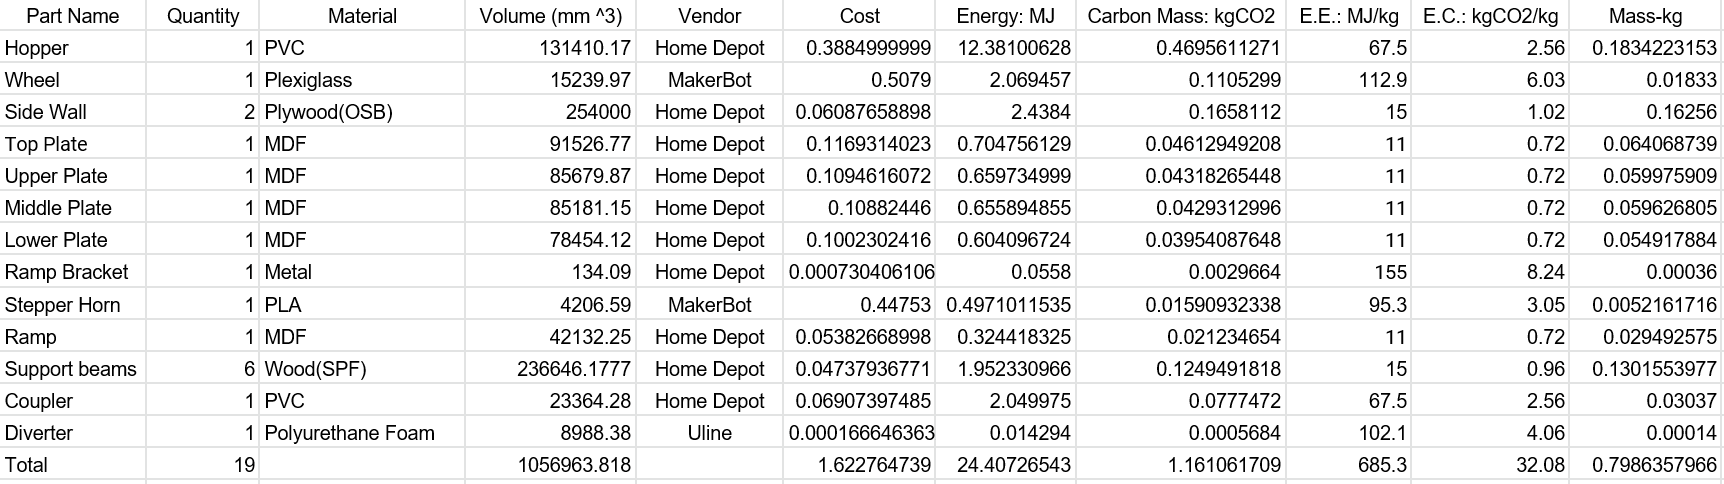
\includegraphics[width=\textwidth]{billofmaterials.png}\\
    \small{\textbf{Figure 5.4.1.1} - Bill of Materials}\\~\\
\end{center}


\subsubsection{Environmental Impact}

The total embodied energy and carbon of the device are 24.407 Megajoules and 1.16 grams CO$_2$, respectively. These values are relatively very low when compared to the global EE and EC of industrial and travel phenomenon. The embodied energy and carbon mass of every part can be found in the Bill of Materials. The part with the highest carbon mass footprint is the hopper, this is due to a relatively medium range carbon coefficient and large mass. The hopper is also the part with the greatest energy used to compose as it’s embodied energy is relatively moderate. Many other parts, specifically the metals and plastics had the potential to have a higher amount of carbon mass and energy as they had relatively high embodied energies and carbon coefficients but were stopped due to a relatively low use of the material.

\newpage
\section{Device Testing}
This section of the report highlights the details of the testing period and the improvements made during the construction process as a result of tests.\\

The first prototype of code involved using many if-else conditions and had a large amount of boolean expressions. The values for testing the balls were spread out, and the structure of the code was very repetitive. The second iteration of the code was made more streamlined by incorporating subfunctions and nested for loops to complete the same task more quickly. Additionally, all information for the balls was stored in custom-defined structs so that the process for checking the balls was more iterative and didn’t require code that was as long.\\

One of the issues the group noticed while testing the code was with the code for the stepper movement. Because the device uses a 3-location system, the stepper motor needed to rotate 120 degrees every rotation. However, the stepper motor uses a PWM signal out of 2048, which is not divisible by 3. Over time, the slight amount of offset from a full rotation would cause the wheel to become misaligned from the holes cut in the fixed plates. To solve this problem, the code uses a modulo 3 system to make sure that the balls are rotated twice by slightly over 120 degrees and once by slightly under 120 degrees so that every 3 rotations adds up to 360 degrees.\\

Another issue was with the power supply. Our initial plan was to run the motors off the power from the Arduino, but the current draw from the servo and stepper was too large and would cause issues with the color sensor shutting off and the motors not functioning properly. To solve this problem, a separate 5V board powered by a 9VDC power supply was used to run electricity to the motors, with power from the Arduino being reserved for the LED and the color sensor.\\

The biggest issue the group encountered was balls getting stuck in certain spots. The first point of issue was from loading in from the hopper. To solve this, a coupler was added with a small diverter made of foam that would funnel the balls to a specific spot instead of letting them roll around the pipe freely. This solution greatly reduced the amount of jamming when loading. The balls also got stuck when they were rotated by the wheel, which sometimes caused them to push the wheel off center and sometimes even pop it off. Different methods such as smoothing the surface area and changing the height of the wheel were tried, but the final design included adding small wooden pieces against the holes in the wheel. This design increased the contact area on the ball, as well as reducing the space it could slip into, which greatly reduced jamming on the rotation platform.\\

Unfortunately, due to time constraints, the group was unable to adequately test the project, so we were unable to produce any experimental data. There were many issues with the balls jamming which prevented us from completing a full test cycle. However, we were able to learn many lessons from this project which will help us with future projects.



\newpage
\section{Conclusions}
To conclude the final design is able to function appropriately with the hardware and software to achieve the main objective and sub-objectives. It is able to do this through the functions that it was designed to do. The cost and energy and carbon footprints of the device are low as the device did not utilize a relatively great amount of material. Multiple issues with the running of the device did occur but they were solvable through creative modifications. Examples include, the addition of a coupler between the device and the hopper, the opening of the hole through which the ball goes to on its way to the rotary wheel, the power supply of the Arduino motors and the rotation angle of the rotary wheel. However, the basic concept of the final design was not altered. One of the main limitations on the determination of environmental impact of the device was that the embodied energy and carbon coefficient of many of the hardware and software parts was difficult to assess as they are composed of multiple materials. The final design was still in need of multiple changes from when it was first selected through the comparison chart. Most of these problems stem from actual application to the physical device issues, small imperfections in the manufacturing of the parts would lead to problems like the jamming of the rotary wheel or the rubber balls. The team found that dependence on a complex code is very perilous as finding the issue with the code could become more difficult then recreating it. \\

In the future, perhaps less emphasis could be placed on the complexity of the code. In general, it is better for the physical design of the device and the code to be as least complex as possible as application problems usually occur and the designs that are simpler are much more easily solved. A possible improvement in the project could be to utilize a software that could model the functions of the device so that the designers can see any possible issues with the design in application. Another suggestion is to give more leniency on the number of designs that could be created. If more designs were created the team could find the device that has less of a susceptibility to application problems. It is somewhat difficult to visualize this susceptibility in each of the top devices when the design concept is only an idea. Perhaps it would help if more attention was placed to the coding software for the color sensor and movement of motors earlier in the project so that more time can be placed on other aspects of the project such as the physical device design. If there were less limitation through the form of charging of costs on 3D printing, laser cutting, and the environmental impact of the device the primary objective could perhaps have been more achievable with all of the functions of the device being rated higher in terms of their success in achieving the objectives.


\newpage
\appendix
\section*{Appendices}
\section{References}

\begin{enumerate}[start=1,label={[\bfseries \arabic*]}]
    \item C. L. Dym, P. Little, and E. Orwin, “Engineering Design: A Project Based Introduction 4th Edition,” pp. 92.
\end{enumerate}

\section{Code}
\subsection{Screenshots of Code}

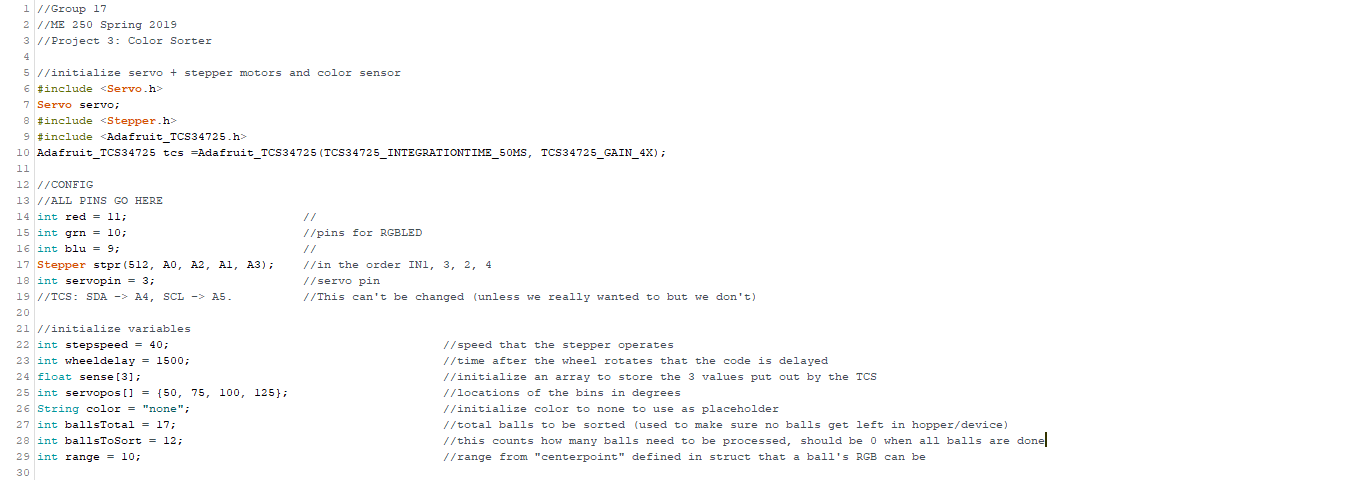
\includegraphics[width=\textwidth]{Screenshot_96.png}\\
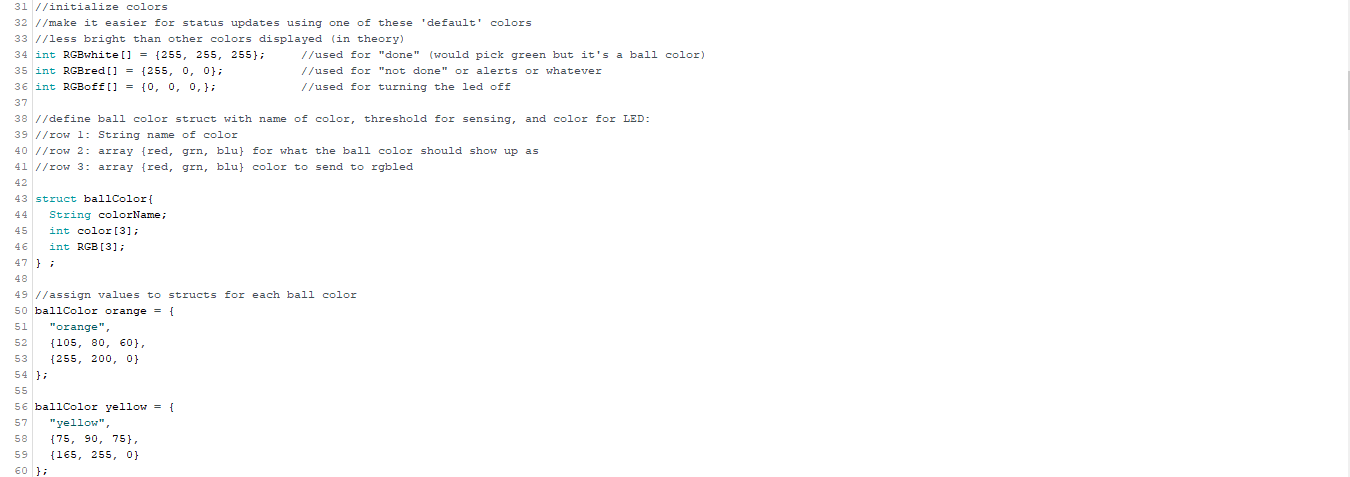
\includegraphics[width=\textwidth]{Screenshot_97.png}\\
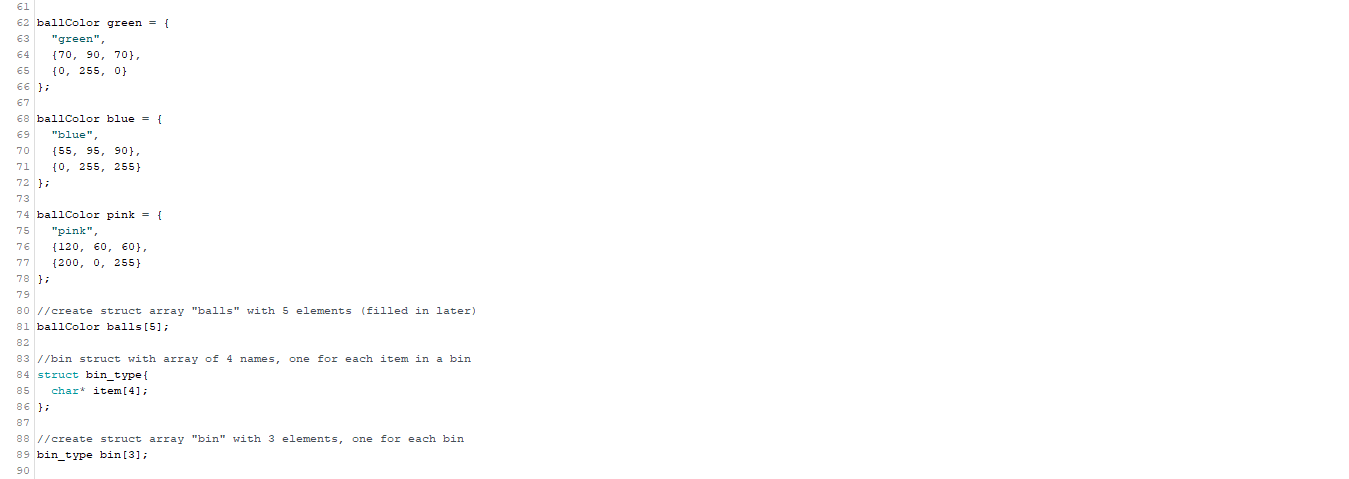
\includegraphics[width=\textwidth]{Screenshot_98.png}\\
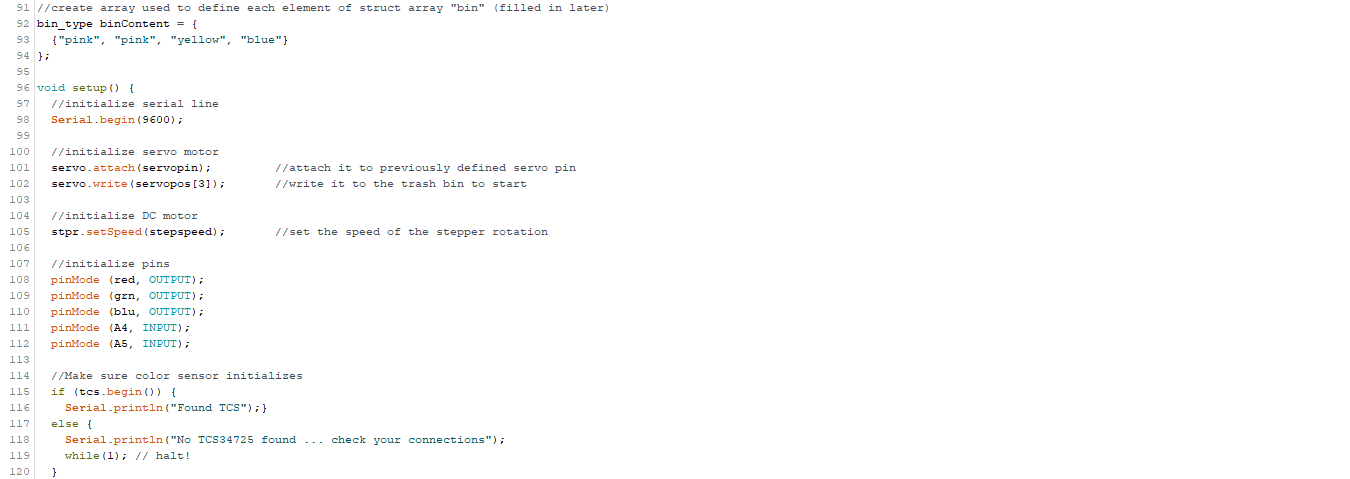
\includegraphics[width=\textwidth]{Screenshot_99.png}\\
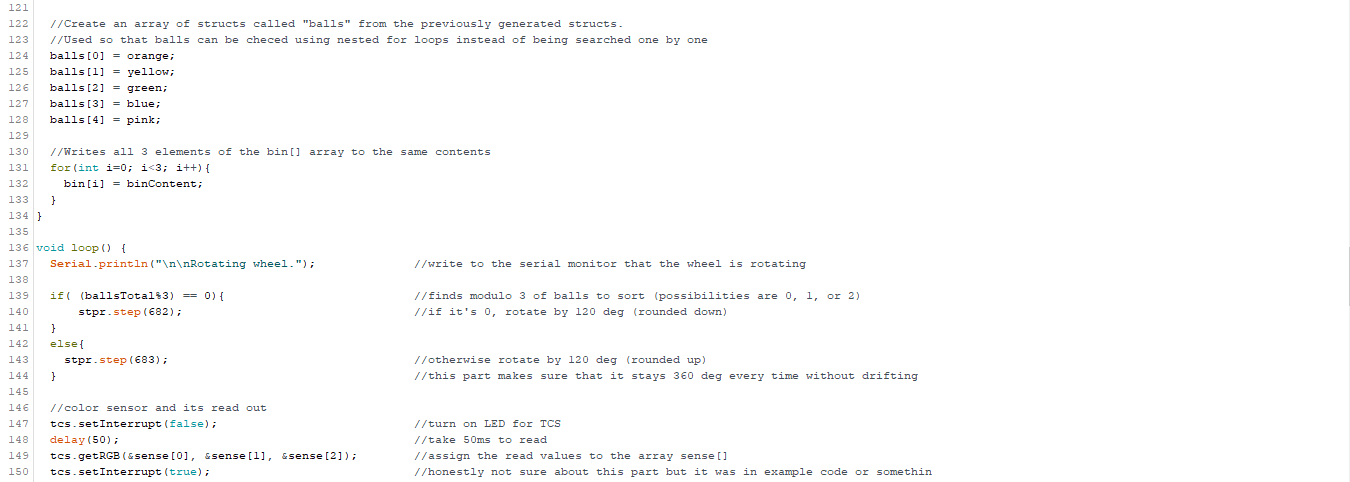
\includegraphics[width=\textwidth]{Screenshot_100.png}\\
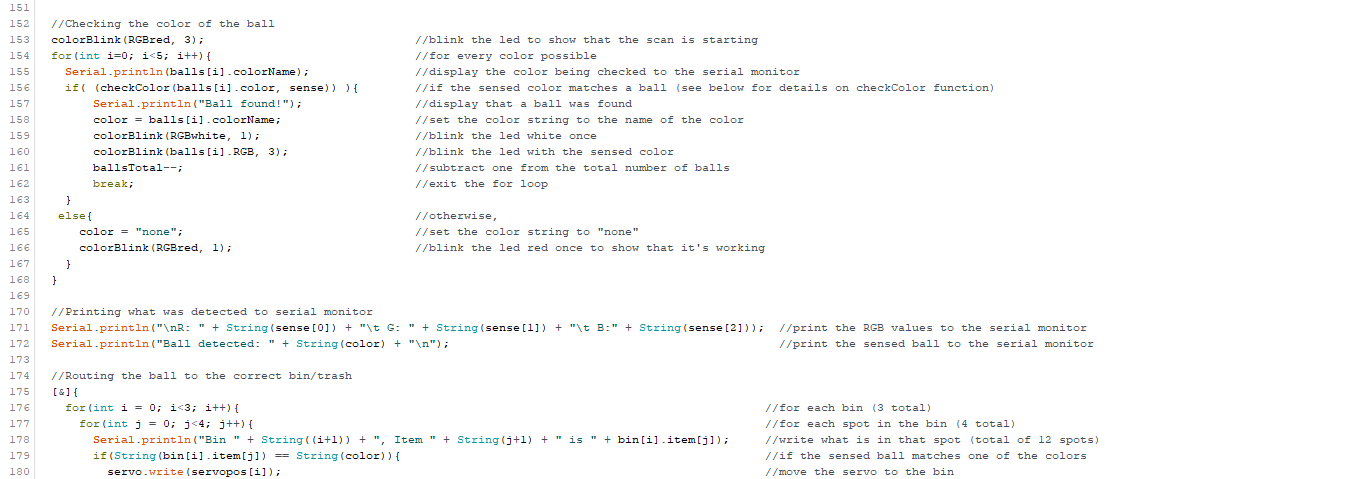
\includegraphics[width=\textwidth]{Screenshot_101.png}\\
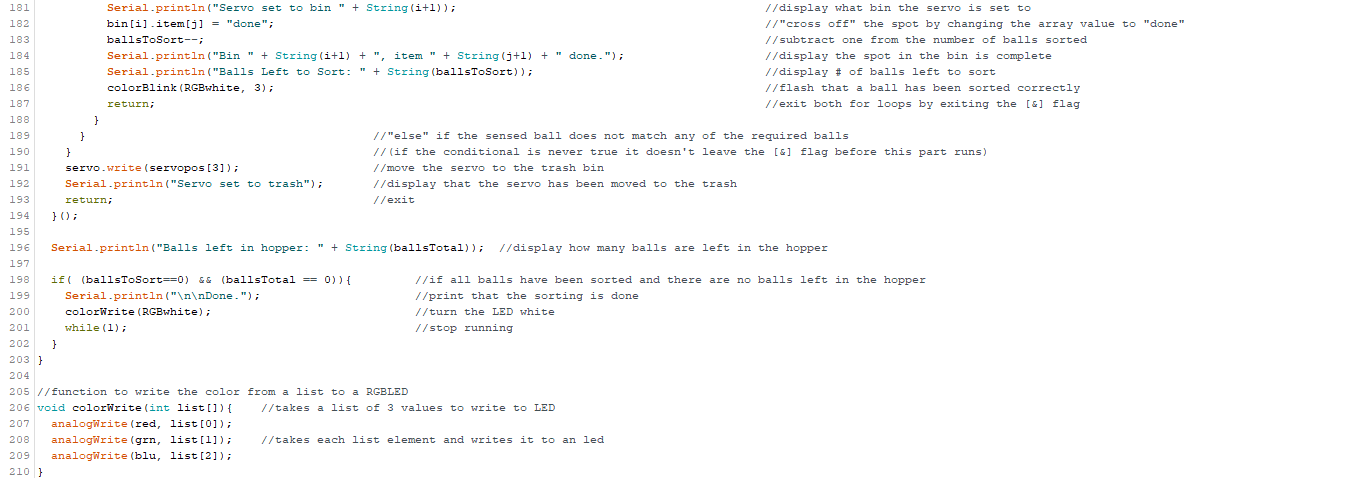
\includegraphics[width=\textwidth]{Screenshot_102.png}\\
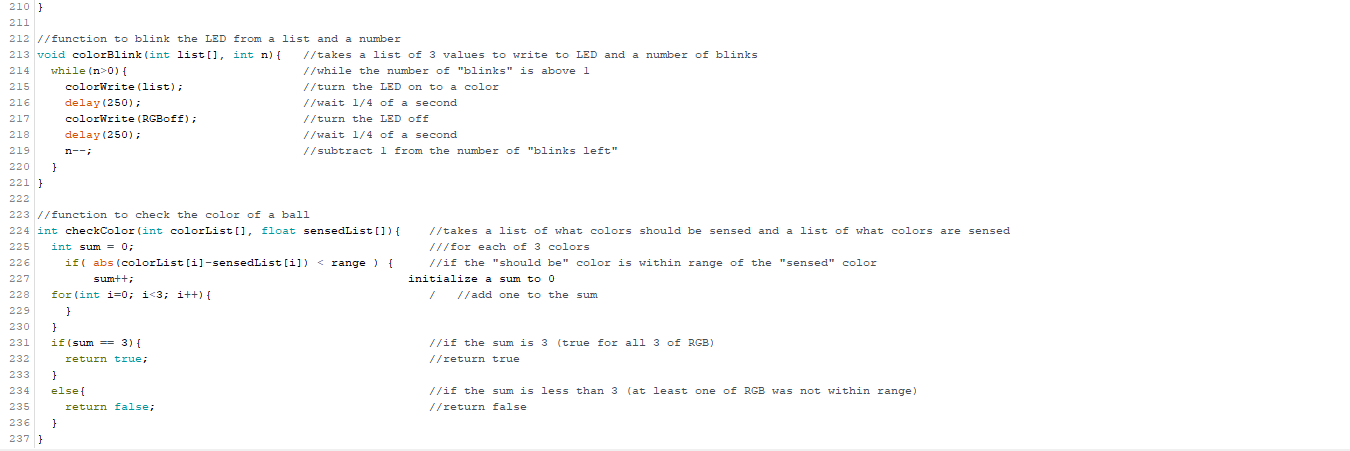
\includegraphics[width=\textwidth]{Screenshot_103.png}\\

\subsection{GitHub}
    Code for this project was maintained in a GitHub repository by Hammad Imam. The main Arduino code used in this project can be seen in more detail \href{https://github.com/himam99/ME250-Proj3/blob/master/Code/me250_proj3_code/me250_proj3_code.ino}{here.} Other code used in the development and testing of this project can be found \href{https://github.com/himam99/ME250-Proj3/tree/master/Code}{here.} Any questions about the GitHub repository can be sent to himam4@uic.edu.
    
\section{CAD}
\subsection{Sources}

All CAD work for this project was done in SolidWorks. CAD models for the stepper, servo, and TCS were found on GrabCAD.

\subsection{Additional Files}

All drawings for the ``As Built" design are given above. The original part and assembly files, as well as the files for previous iterations of the design, can be seen \href{https://github.com/himam99/ME250-Proj3/tree/master/CAD}{here.}

\end{document}
